
%%%%%%%%%%%%%%%%%%%%%%%%%%%%%%%%%%%%%%%%%%%%%%%%%%%%%%%%%%%%%%%%%%%%%%%%%%%%
%%%%%%%%%%%%%%%%%%%%%%%%%%%%%%%%%%%%%%%%%%%%%%%%%%%%%%%%%%%%%%%%%%%%%%%%%%%%
%%%%%%%
%%%%%%% APPTENDIX
%%%%%%%
%%%%%%%
%%%%%%% The Contagion of Drug Violence: 
%%%%%%% Spatio-temporal Dynamics of the Mexican War on Drugs
%%%%%%%
%%%%%%% Compiled in: www.sharelatex.com
%%%%%%%
%%%%%%%%%%%%%%%%%%%%%%%%%%%%%%%%%%%%%%%%%%%%%%%%%%%%%%%%%%%%%%%
%%%%%%%%%%%%%%%%%%%%%%%%%%%%%%%%%%%%%%%%%%%%%%%%%%%%%%%%%%%%%%%

\documentclass[12pt,letterpaper]{article}
\usepackage[utf8]{inputenc}
\usepackage[T1]{fontenc}
\usepackage[margin=2.5cm]{geometry}
\usepackage{amsmath}

\usepackage{endnotes}                       % http://ctan.org/pkg/endnotes
\let\footnote\endnote
\def\footnotetext{\endnotetext[\number\numexpr\value{endnote}+1]}
\let\footnotemark\endnotemark


\usepackage{array}                          %For centering justified text in tables%
\usepackage{setspace}                       % To shrink space between lines %
\singlespacing                              % Uncomment for single spacing%

\usepackage{latexsym}
\usepackage{longtable}                      % For tables across multiple pages
\usepackage{multirow}                       % For tables with a cell covering multiple rows
\usepackage{lscape}                         % Horizontal page %
\usepackage{chngcntr}
\usepackage{caption}
\usepackage{longtable}
\usepackage{float}                          % For tables and graphs  %
\usepackage[capposition=top]{floatrow}      %For adding a note below a figure%
\usepackage{booktabs,caption,fixltx2e}      %For adding a note below a figure%
\usepackage[flushleft]{threeparttable}      %For adding a note below a figure%
\usepackage{subfigure}
\usepackage[demo]{graphicx}
\usepackage{caption}
\usepackage{subcaption}

\usepackage{multirow}
\usepackage[hidelinks=true]{hyperref}
\usepackage[hyphenbreaks]{breakurl}

\usepackage{natbib}   % Bibliography %
\setlength{\bibsep}{1.9 pt} %To reduce space between lines in the bilbiography%

\usepackage[all,defaultlines]{nowidow}      % Prevents widows and orphans %



\newcommand{\N}{\mathrm{N}}



%%%%%%%%%%%%%%%%%%%%%%%%%%%%%%%%%%%%%%%%%%%%%%%%%%%%%%%%%%%%%%%
%%%%%%%%%%%%%%%%%%%%%%%%%%%%%%%%%%%%%%%%%%%%%%%%%%%%%%%%%%%%%%%

%\title{ Appendix}
%\date{\vspace{-5ex}}

\title{ Online Appendix   \\ The Contagion of Drug Violence. Spatio-temporal Dynamics of the Mexican War on Drugs}

\author{Javier Osorio}

\date{January 2015}







%%%%%%%%%%%%%%%%%%%%%%%%%%%%%%%%%%%%%%%%%%%%%%%%%%%%%%%%%%%%%%%
%%%%%%%%%%%%%%%%%%%%%%%%%%%%%%%%%%%%%%%%%%%%%%%%%%%%%%%%%%%%%%%
\begin{document}

\maketitle


The Online Appendix of the manuscript ``The Contagion of Drug Violence. Spatio-temporal Dynamics of the Mexican War on Drugs'' is structured in four sections.  The first part indicates the coding rules used for developing the Organized Crime Violence Event Data (OCVED) data set. This section also reports the information sources consulted in the data collection process, discusses possible concerns of bias from the information sources and mentions the actor and verb categories used for event coding using Eventus ID. The second section presents the time series and reports the descriptive statistics of the event data contained in OCVED. It also shows the summary statistics of other covariates. In addition, this section indicates the information source for each covariate and reports the original unit of analysis of each variable before being imputed at the municipal-weekly basis in this study. The third section reports the correlation between OCVED and other databases of violence in Mexico. Results show that the measure of violence among DTOs analyzed in this study is highly correlated with homicide data reported by alternative sources. Finally, the fourth section replicates the regression results reported in the manuscript and offers several robustness tests considering alternative lags of law enforcement data.  




%%%%%%%%%%%%%%%%%%%%%%%%%%%%%%%%%%%%%%%%%%%%%%%%%%%%%%%%%%%%%%%%%%%%%%%%%%%%%%%%%%%%%%%%%%%%%%%%%%%%%%%%
%%%%%%%%%%%%%%%%%%%%%%%%%%%%%%%%%%%%%%%%%%%%%%%%%%%%%%%%%%%%%%%%%%%%%%%%%%%%%%%%%%%%%%%%%%%%%%%%%%%%%%%%
%  SECTION
\section{OCVED coding protocol}



\subsection{Coding rules}

To select the appropriate news reports, research assistants were trained to apply the following criteria for inclusion and exclusion of news reports:

\textbf{Inclusion criteria}: The main objective of the selection criteria is to select reports providing information about events of organized criminal violence. The instructions for selection were:


\begin{enumerate} %\itemsep-0.50em
    \item Include reports of events associated with violent actions such as armed clashes, murders, killings, shootings, ambushes, attacks, assassination attempts, wounding, kidnapping, torture or mutilation that involve the participation of presumed members of criminal organizations as perpetrators or victims.
    \item Some reports of violent actions may not explicitly mention the participation of organized criminals as perpetrators or victims, but these events should be included if their \emph{modus operandi} involves one or more of the following characteristics: 
        \begin{itemize} %\itemsep-0.05em
        \item Use of assault weapons.
        \item Two or more victims.
        \item Signs of mutilation or torture in the victims.
        \item Execution-style killings (\emph{coup de gr\^{a}ce}, known in Spanish as ``\emph{tiro de gracia}'').
        \item Participation of at least one group of armed men (commandos or death squads).
        \item Participants traveling in convoys of vehicles (usually SUVs, pick-up trucks or luxury vehicles).
        \item Signs, marks or messages (``\emph{narcomensajes}'') associated with organized crime.
        \item Bodies discovered in clandestine mass graves, wrapped in blankets (``\emph{ensarapados}''), found in the trunk of abandoned vehicles (``\emph{encajuelados}'') or in containers (``\emph{entambados}'').
        \end{itemize}
    
    This set of characteristics is based on the criteria used by the Mexican government for classifying a homicide as being presumed to be associated with organized crime. See \citet{SistemaNacionaldeSeguridadPublica2011}.
        
    \item Include reports of events associated with kidnapping, extortion or money laundering even though organized crime or drug trafficking organizations are not explicitly mentioned in the report. 
    \item Include reports of events associated with law enforcement actions by state security forces when conducting operations against criminal organizations. Law enforcement actions can be violent or non-violent: 
        \begin{itemize} \itemsep-0.4em
        \item Violent law enforcement refers to events in which the state's coercive apparatus uses force to deliberately inflict physical damage on suspected members of criminal organizations. These actions may include events in which the state attacked suspected organized criminals or repelled a criminal act of aggression, or events in which security forces wounded or killed one or more suspected organized criminals.
        \item Non-violent law enforcement refers to state actions that resulted in the arrest of suspected members of criminal organizations or the confiscation of drugs, weapons or assets (e.g.\ money, real estate, vehicles, items) used for their illegal activities.
        \end{itemize}
\end{enumerate}



The elements of the inclusion criteria provided the main guidelines for selecting relevant reports associated with drug violence. However, the exclusion criteria was equally important to guarantee the quality of information included in the database. 

\textbf{Exclusion criteria}: This research is exclusively focused on \emph{events} associated with organized crime violence. In consequence, the process of information gathering should exclude reports containing the following kind of information:

\begin{enumerate} %\itemsep-0.05em
    \item Exclude reports about speeches, declarations, discourses, opinions, newspaper editorials or public statements made about events associated with organized crime violence. 
        \begin{itemize} %\itemsep-0.05em
        \item This criterion is crucial. Drug violence receives considerable media attention and lots of people talk about it. However, this research is strictly focused on events (facts and episodes), not on what people say about those events. 
        \end{itemize}
    \item Exclude reports associated with deaths, injuries or material damage caused by any of the following:
        \begin{itemize} %\itemsep-0.4em
        \item  Attacks by insurgent groups (e.g.\ Ejercito Zapatista de Liberaci\'{o}n Nacional, EZLN, or Ej\'{e}rcito Popular Revolucionario, EPR) or any other radical group with political motivations.
        \item  Accidents, natural disasters, diseases or attacks by animals.
        \item  Crimes of passion.
        \item  Street level crime and minor offenses (e.g.\ burglary, theft, simple assault, robbery). 
        \item  Violent criminal behavior that does not have the characteristics mentioned in the inclusion criteria (e.g.\ a police officer shot during a robbery of a convenience store).
        \item  Events of organized crime violence occurring outside Mexico (e.g.\ clashes between Zetas and local drug dealers in Guatemala).
        \item  Violence associated with protests, riots or contentious tactics undertaken by groups with social, political, economic or environmental demands against the government.
        \end{itemize}
    \item Exclude government reports summarizing the activities conducted or results achieved over aggregated periods of time (e.g.\ monthly or annual reports). 
\end{enumerate}

The systematic application of the inclusion and exclusion criteria helped identifying valid events of organized criminal violence.








%%%%%%%%%%%%%%%%%%%%%%%%%%%%%%%%%%


\subsection{Information sources}

Table \ref{number_of_news_reports} indicates the number of news reports collected by type of source. Table \ref{tab:ocved_info_sources} shows the list of information sources used to build OCVED.




%%%%%%%%%%%%%%%%%%%%%%%%%%%%%%%%%%


\begin{table}[h!]
\small
%\begin{spacing}{-0.8}
    \caption{Number of news reports gathered by source}
    \label{number_of_news_reports}
%\end{spacing}
\begin{spacing}{0.95}
    \centering
    \begin{tabular}{|l|r|c|}
        \hline
Information source  &  Num. of news reports  & Percentage by type   \\
\hline \hline
Police  &  1,572  & 3.76\%    \\
Navy  &  421  & 1.01\%   \\
Attorney General   &  3,328  & 7.95\%   \\
State Attorney General   &  12,728  & 30.42\%   \\
Army  &  3,026  & 7.23\%   \\
National press  &  10,849  & 25.93\%   \\
Local press  &  9,914  & 23.7\%    \\
\hline
Total   &  41,838  & 100\%   \\
\hline  
\end{tabular}
\end{spacing}
\end{table}





%%%%%%%%%%%%%%%%%%%%%%%%%%%%%%%%%%

\begin{table}[h!]
\small
%\begin{spacing}{-0.8}
    \caption{List of information sources}
    \label{tab:ocved_info_sources}
%\end{spacing}
\begin{spacing}{0.95}
    \centering
    \begin{tabular}{|ll|}
    \hline
    
\multicolumn{2}{|l|}{\textbf{Federal government agencies: 4  }}     \\
\hline
%\multicolumn{2}{|p{15cm}|}{ Secretar\'{\i}a de la Defensa Nacional (SEDENA),  Secretar\'{\i}a de Seguridad P\'{u}blica (SSP),  Secretar\'{\i}a de Marina Armada de M\'{e}xico (SEMAR), Procuradur\'{\i}a General de la Rep\'{u}blica (PGR) }  \\        \hline
\multicolumn{2}{|p{15cm}|}{ Secretar\'{\i}a de la Defensa Nacional,  Secretar\'{\i}a de Seguridad P\'{u}blica,  Secretar\'{\i}a de Marina Armada de M\'{e}xico, Procuradur\'{\i}a General de la Rep\'{u}blica}  \\
        \hline
        
\multicolumn{2}{|l|}{\textbf{Local government agencies: 32  }}     \\
\hline
\multicolumn{2}{|p{15cm}|}{State Attorney Generals for all states: Procuradur\'{\i}as Estatales}   \\
\hline

\multicolumn{2}{|l|}{\textbf{National level newspapers and magazines: 11}}     \\
\hline
\multicolumn{2}{|p{15cm}|}{Servicio Universal de Noticias, El Economista, El Financiero, Exc\'{e}lsior,  Notimex - Nacional, Reforma, La Jornada, El Sol de M\'{e}xico, Milenio Diario, Revista Proceso, La Cr\'{o}nica de Hoy }  \\
\hline

\multicolumn{2}{|l|}{\textbf{Local level newspapers: 58  }}     \\
\hline
Aguascalientes  &  El Sol - Regional Newspapers   \\
Baja California  &  \multicolumn{1}{p{11cm}|}{El Mexicano,  El Sol - Regional Newspapers,  La Voz de la Frontera}   \\
Baja California Sur  &  El Sudcaliforniano   \\
Campeche  &  Diario de Yucat\'{a}n - Campeche   \\
Chiapas  &  Notimex - Estados  \\
Chihuahua  &  \multicolumn{1}{p{11cm}|}{Diario de Ju\'{a}rez, El Diario de Chihuahua,  El Diario de Delicias, El Diario de Nuevo Casas Grandes,  El Diario de Parral, El Sol - Regional Newspapers }  \\
Coahuila   &  La Opini\'{o}n, Milenio de Torre\'{o}n, El Sol - Regional Newspapers   \\
Colima  &  Notimex - Estados \\
Distrito Federal  &  El Sol - Regional Newspapers   \\
Durango  &  El Sol - Regional Newspapers   \\
Estado de M\'{e}xico  &  Milenio Estado de M\'{e}xico   \\
Guanajuato  &  \multicolumn{1}{p{11cm}|}{Peri\'{o}dico A.M. Celaya, Peri\'{o}dico A.M. Guanajuato, Peri\'{o}dico A.M. Irapuato, Peri\'{o}dico A.M. La Piedad,  Peri\'{o}dico A.M. Le\'{o}n, Peri\'{o}dico A.M. San Francisco del Rinc\'{o}n,  Milenio - Le\'{o}n, El Sol - Regional Newspapers }  \\
Guerrero  &  El Sol - Regional Newspapers   \\
Hidalgo  &  Milenio Pachuca, El Sol - Regional Newspapers   \\
Jalisco  &  Mural - Newspaper,  Milenio Guadalajara   \\
Michoac\'{a}n  &  El Sol - Regional Newspapers   \\
Morelos  &  \multicolumn{1}{p{11cm}|}{Ecos de Morelos - La Uni\'{o}n de Morelos, El Sol - Regional Newspapers }  \\
Nayarit  &  Notimex - Estados \\
Nuevo Le\'{o}n  &  Milenio Diario de Monterrey,  El Norte - Newspaper   \\
Oaxaca  &  Notimex - Estados \\
Puebla  &  Milenio Puebla , El Sol - Regional Newspapers   \\
Quer\'{e}taro  &  \multicolumn{1}{p{11cm}|}{Diario de Quer\'{e}taro, El Occidental,  El Sol - Regional Newspapers }  \\
Quintana Roo  &  Notimex - Estados \\
San Luis Potos\'{\i}  &  El Sol de San Luis, El Sol - Regional Newspapers   \\
Sinaloa  &  El Sol - Regional Newspapers   \\
Sonora  &  Notimex - Estados \\
Tabasco  &  Milenio Villahermosa   \\
Tamaulipas  &  Milenio Diario de Tampico ,  El Sol - Regional Newspapers   \\
Tlaxcala  &  El Sol - Regional Newspapers   \\
Veracruz   &  Milenio Xalapa, El Sol - Regional Newspapers   \\
Yucat\'{a}n  &  Diario de Yucat\'{a}n   \\
Zacatecas  &  El Sol - Regional Newspapers   \\
\hline  
\end{tabular}
\end{spacing}
\end{table}




%%%%%%%%%%%%%%%%%%%%%%%%%%%%%%%%%%

\clearpage

\subsection{Concerns of bias from information soruces}

As indicated in Tables \ref{tab:ocved_info_sources} and \ref{number_of_news_reports}, the sources of information considered in this research are highly fragmented. Even those types of sources that seem to contribute a substantial proportion of news reports--such as the State Attorney General with 30.42\%, national newspapers with 25.93\% or local press with 23.7\% of reports--comprize dozens of uncoordinated and independent reporting agencies--there are 32 autonomous State Attorney offices, 11 national newspapers and 58 state newspapers. In this way, the variety of information sources reduces concerns of systematic bias induced by a predominant source. 

As suggested by \citet{Andreas2010}, competition between government agencies for budgetary allocations provides incentives for different law enforcement branches to report their activities as a way of signaling good performance. This incentive reduces concerns for systematic underreportiong of drug related events by the government.  

Scholars such as \citet{Hallin2000} warn about the high levels of media control imposed by the government during the dominance era of the Institutional Revolutionary Party (PRI). During this period, journalists were mostly passive and self-censored. In consequence, news reports were generally  aligned with the official discourse. As indicated by \citet{Lawson2002}, the process of democratic transition deeply redefined the relationships between media and the government. The gradual process of political opening initiated in the 1980s at the subnational level and culminating with the Presidential alternation in 2000 favored the emergence and consolidation of a proactive and independent free media sector. The extent of media freedom in Mexico after the democratic transition and the plurality of national and local newspapers considered in this study reduce concerns of effective and systematic media control by the government.   


%%%%%%%%%%%%%%%%%%%%%%%%%%%%%%%%%%


\subsection{Coding event data using Eventus ID}

The development of OCVED relies on Eventus ID, a novel software for automated event coding from text written in Spanish \citep{Osorio2014}. Eventus ID uses a set of actors and verbs dictionaries to recognize specific words in news reports, thus identifying the key components of event data. In a basic level, an event can be defined as a set of elements providing information about someone doing something to someone else. Events are composed of three key elements:
\begin{description}
    \item[Source:] Refers to the actor or perpetrator of the action. Eventus ID uses proper nouns to identify the actors mentioned in the text.
    \item[Action:] Indicates the specific action carried out by the source. Actions are identified by the system as verb phrases in the text.
    \item[Target:] Refers to the actor towards or upon whom the perpetrator carried out an action. Eventus ID uses the list of actors to identify the target of the event.
\end{description}



The coding protocol impemented in this research considers the following actor categories:

\begin{itemize} \itemsep-0.4em
    \item Federal government: refers to a variety of government agencies in the Executive, Congress and Judicial branches, as well as the name of key individuals occupying those positions at the federal level.     
    \item Coercive apparatus: relates to a broad range of institutions, individuals and special groups in the Army, Navy, Air Force and different Police forces at the federal, state and municipal levels. 
    \item Local government: refers to the Governor, Mayor and representatives at the local government.    
    \item Individuals: includes a broad range of proper nouns referring to civilians or individuals.
    \item Victims: indicates civilians who were victims of violence, either perpetrated by criminal organizations or by government security forces.                 
    \item Criminal organizations: includes an exahusitive list of names of criminal organizations and their most prominent leaders. 
    \item Criminal assets: refers to a broad list of aerial, maritime and terrestrial vehicles, as well as properties and real estate presumably belonging to criminal organizations.        
    \item Drugs: relates to a detailed list of illegal drugs.                  
    \item Weapons: refers to a variety of weapons of different types and calibers (e.g pistols, shotguns or rifles), as well as other military, tactic or communication equipment.                
\end{itemize}



In addition to the list of actors, the automated coding protocol relies on a list of verb phrases to identify the actions being conducted. These are the verb categories considered in this research: ``attack,'' ``detect,'' ``shoot,'' ``seize,'' ``clash,'' ``eradicate,'' ``arrest,'' ``kidnap,'' ``raid,'' ``burn,'' ``wound,'' ``torture,'' ``mutilate,'' and ``kill.'' 


Based on the previous definitions, OCVED aggregates event data to conform the following categories:

\begin{itemize} \itemsep-0.4em
    
    \item Violence between DTOs: Considers episodes where the source and the target are members of criminal organizations, individuals or victims and the event is associated with the following kinds of actions:  ``attack,'' ``shoot,'' ``clash,''  ``kidnap,''  ``burn,'' ``wound,'' ``torture,'' ``mutilate,'' and ``kill.''   
        
        \begin{itemize}
        \item For example, the sentence ``members of the Sinaloa cartel clashed with a group hitmen of the Zetas organization'' would lead to this kind of event. 
        \end{itemize}
    
    \item Violent law enforcement:  Considers episodes where the source of the action are members of the coercive apparatus, federal government or local government and the target are individuals or members of criminal organizations and the event is associated with the following kinds of actions:  ``attack,''  ``shoot,''  ``clash,'' ``arrest,''  ``raid,'' ``burn,'' ``wound,''  and ``kill.''
        
        \begin{itemize}
        \item For example, the sentence ``troops of the 2nd infantry battalion shot down a presumed member of a criminal group'' would lead to this kind of event. 
        \end{itemize}
        
    \item Arrests:  Considers episodes where the source of the action are members of the coercive apparatus, federal government or local government, the target are individuals or members of criminal organizations and the event is associated with the action: ``arrest.'' 
        
        \begin{itemize}
        \item For example, the sentence ``elements of the federal police arrested a drug dealer'' would lead to this kind of event. 
        \end{itemize}
        
    \item Seizures of assets: Considers episodes where the source is a member of the state's coercive apparatus, the federal or local government, the target is a criminal asset and the event is associated with the action: ``seize.'' 
        
        \begin{itemize}
        \item For example, the sentence ``the Navy confiscated the speedboat'' would lead to this kind of event. 
        \end{itemize}
        
    \item Seizures of drugs:  Considers episodes where the source of the action are members of the coercive apparatus, federal government or local government and the target are individuals or members of criminal organizations and the event is associated with the following kinds of actions:  ``detect,'' ``seize,'' ``eradicate,'' and ``burn.''
        
        \begin{itemize}
        \item For example, the sentence ``members of the state police force seized a package with 25 kgs of cocaine'' would lead to this kind of event. 
        \end{itemize}
        
    \item Seizures of weapons: Considers episodes where the source is a member of the state's coercive apparatus, the federal or local government, the target is weapon and the event is associated with the action: ``seize.'' 
        
        \begin{itemize}
        \item For example, the sentence ``members of special forces confiscated an arsenal of assault wapons'' would lead to this kind of event. 
        \end{itemize}
        
    \item Violent retaliation: Considers episodes where the source is a member of a criminal organizations or an individual, the target is  a member of the coercive apparatus, federal government or local government and the event is associated with the following kinds of actions:  ``attack,'' ``shoot,'' ``clash,''  ``kidnap,''  ``burn,'' ``wound,'' ``torture,'' ``mutilate,'' and ``kill.'' This variable is not included in this study but is part of OCVED event data.        
        \begin{itemize}
        \item For example, the sentence ``a group of heavily armed attacked a military convoy'' would lead to this kind of event. 
        \end{itemize}
        
\end{itemize}



%%%%%%%%%%%%%%%%%%%%%%%%%%%%%%%%%%%%%%%%%%%%%%%%%%%%%%%%%%%%%%%%%%%%%%%%%%%%%%%%%%%%%%%%%%%%%%%%%%%%%%%%
%%%%%%%%%%%%%%%%%%%%%%%%%%%%%%%%%%%%%%%%%%%%%%%%%%%%%%%%%%%%%%%%%%%%%%%%%%%%%%%%%%%%%%%%%%%%%%%%%%%%%%%%

\clearpage

%%%%%%%%%%%%%%%%%%%%%%%%%%
%  SECTION
\section{Descriptive statistics and additional variable information}

Figure \ref{fig:event_data_NM} shows the temporal trends of the different types of event data used in this research. Table \ref{tab:descriptive_OCVED} presents the descriptive statistics of the event data variables included in OCVED; the data is reported at the municipal-week level. Table \ref{tab:descriptive_interactions} shows the descriptive statistics of different law enforcement variables when interacted with different measures of criminal groups presence and road density. In addition, Table \ref{tab:descriptive_covariates} reports the descriptive statistics of all other covariates considered in this study. Finally, Table \ref{tab:info_sources} indicates the sources of information of the covariates as well as their original level of aggregation before being interpolated at the municipal-weekly level.


The different plots in Figure \ref{fig:event_data_NM} present the time series of violence between DTOs, violent enforcement, arrests, and seizures of drugs, assets, and weapons. For illustrative purposes, data in this figure is aggregated at the national-monthly level, but the statistical analysis is conducted at the municipality-week unit of analysis.  Panel (a) shows a dramatic and sustained increase of violence between DTOs in the second half of the decade. Panels (b) through (f) also show a consistent increase in the tactics deployed by the state to fight crime after President Calder\'{o}n launched the war on drugs in December 2006. Although violence is not frequently employed by government authorities, the use of this tactic rose sharply after 2007, as illustrated in Panel (b). The data shows that authorities primarily rely on arrests and drug seizures to fight DTOs. As indicated in Panels (c) and (d) respectively, despite some fluctuations in the first half of the decade, both tactics rose dramatically from 2007 on. Confiscation of criminal assets, shown in Panel (e), and seizure of weapons, Panel (f), are used less than detentions and drug interdiction, but the trends show increasing government efforts to confiscate assets and to disarm criminals.    

Figure \ref{fig:number_DTOs} reports the number of municipalities with DTO activity. Panel (a) reports the number of locations in which the news reported the presence of at least one drug trafficking organization. This panel shows a dramatic territorial expansion of criminal groups starting in 2006. In addition, Panel (b) disaggregates the information by distinguishing between \emph{main DTOs} and \emph{secondary DTOs}. The trends indicate a substantial increase of territorial presence of main DTOs around 2006 and a sharp increase of secondary DTOs towards the end of the decade.


%\begin{center}
%   [Insert Figure~\ref{fig:event_data_NM} about here]
%\end{center}

\newpage

\begin{figure}[h]
\centering
\subfigure[Violence between DTOs]{
    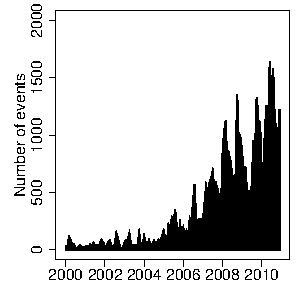
\includegraphics[width=.3\textwidth]{figures/DVD_TS.pdf}
}
\subfigure[Violent enforcement]{
    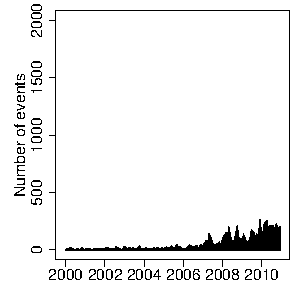
\includegraphics[width=.3\textwidth]{figures/SVD_TS.pdf}
}
\subfigure[Arrests]{
    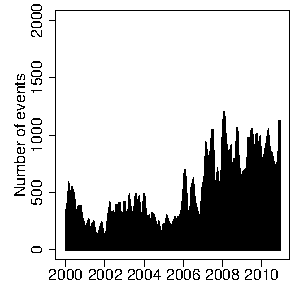
\includegraphics[width=.3\textwidth]{figures/SAD_TS.pdf}
}
\subfigure[Drug seizures]{
    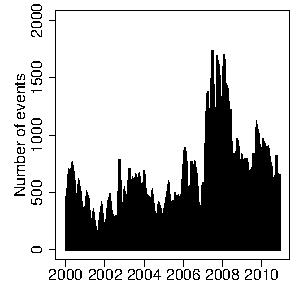
\includegraphics[width=.3\textwidth]{figures/SSD_TS.pdf}
}
\subfigure[Seizures of assets]{
    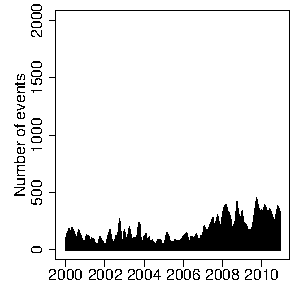
\includegraphics[width=.3\textwidth]{figures/SSA_TS.pdf}
}
\subfigure[Seizures of guns]{
    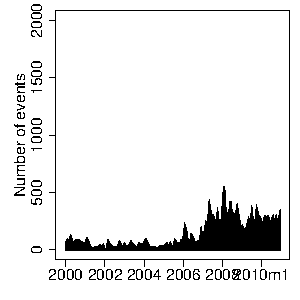
\includegraphics[width=.3\textwidth]{figures/SSG_TS.pdf}
}
\caption{Time series of event data 2000--2010 (national monthly data)}
\label{fig:event_data_NM}
\end{figure}





\begin{figure}[h!]
\centering
\subfigure[All DTOs]{
    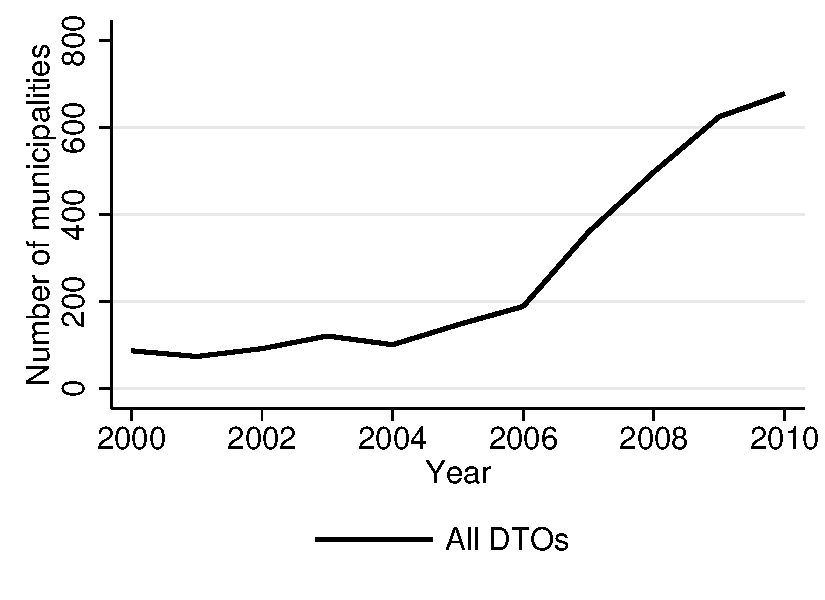
\includegraphics[width=.45\textwidth]{figures/dtos_all_bw.pdf}
}
\subfigure[Main and secondary DTOs]{
    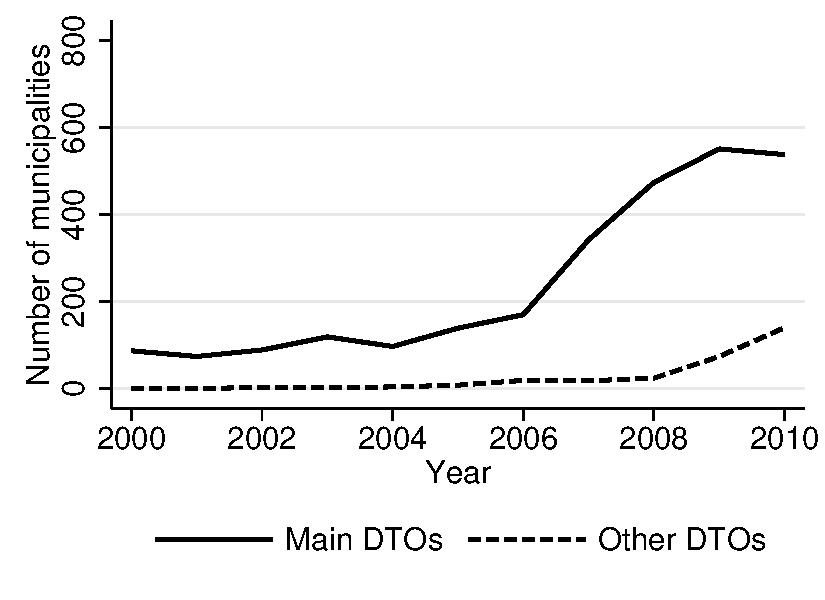
\includegraphics[width=.45\textwidth]{figures/dtos_main_other_bw.pdf}
}
\caption{Number of municipalities with activity of DTOs 2000--2010}
\label{fig:number_DTOs}
\end{figure}






\begin{table}[h!]
\small
%\footnotesize
%\begin{spacing}{-0.8}
    \caption{Descriptive Statistics OCVED (weekly data)}
    \label{tab:descriptive_OCVED}
%\end{spacing}
\begin{spacing}{0.95}
    \centering
    \begin{tabular}{lrrrrr}
    \hline
    

	Variable       	&	Observations	&	Mean	&	Std. Dev.	&	Min	&	Max	 \\	\hline
													
	Violence between DTOs	&	 1,667,624 	&	0.028	&	0.379	&	0	&	48	 \\
	\hspace{1em} Logged	&	 1,667,624 	&	0.013	&	0.126	&	0	&	3.89182	 \\
	\hspace{1em} Lagged 1 	&	 1,665,168 	&	0.028	&	0.378	&	0	&	48	 \\
%	\hspace{1em} Lagged 1 logged	&	 1,665,168 	&	0.013	&	0.126	&	0	&	3.89182	 \\
	\hspace{1em} Lagged 2 	&	 1,662,712 	&	0.028	&	0.378	&	0	&	48	 \\
%	\hspace{1em} Lagged 2 logged	&	 1,662,712 	&	0.013	&	0.126	&	0	&	3.89182	 \\
%	\hspace{1em} Lagged 4	&	 1,657,800 	&	0.028	&	0.374	&	0	&	48	 \\
%	\hspace{1em} Lagged 4 logged	&	 1,657,800 	&	0.013	&	0.125	&	0	&	3.89182	 \\
%	\hspace{1em} Lagged 8 	&	 1,647,976 	&	0.028	&	0.373	&	0	&	48	 \\
%	\hspace{1em} Lagged 8 logged	&	 1,647,976 	&	0.013	&	0.125	&	0	&	3.89182	 \\
    \hspace{1em} Rate (lag 1 - lag 2)	&	 1,662,712 	&	0.000	&	0.398	&	-48	&	48	 \\
		
	Violent enforcement	&	 1,667,624 	&	0.004	&	0.100	&	0	&	34	 \\
%	\hspace{1em} Logged	&	 1,667,624 	&	0.002	&	0.044	&	0	&	3.555348	 \\
%	\hspace{1em} Lagged 1 	&	 1,665,168 	&	0.004	&	0.099	&	0	&	34	 \\
%	\hspace{1em} Lagged 1 logged	&	 1,665,168 	&	0.002	&	0.044	&	0	&	3.555348	 \\
%	\hspace{1em} Lagged 2 	&	 1,662,712 	&	0.004	&	0.099	&	0	&	34	 \\
	\hspace{1em} Lagged 2 logged	&	 1,662,712 	&	0.002	&	0.044	&	0	&	3.555348	 \\
%	\hspace{1em} Lagged 4	&	 1,657,800 	&	0.004	&	0.098	&	0	&	34	 \\
	\hspace{1em} Lagged 4 logged	&	 1,657,800 	&	0.002	&	0.044	&	0	&	3.555348	 \\
%	\hspace{1em} Lagged 8 	&	 1,647,976 	&	0.004	&	0.098	&	0	&	34	 \\
	\hspace{1em} Lagged 8 logged	&	 1,647,976 	&	0.002	&	0.044	&	0	&	3.555348	 \\
												
												
	Arrests	&	 1,667,624 	&	0.038	&	0.448	&	0	&	207	 \\
%	\hspace{1em} Logged	&	 1,667,624 	&	0.020	&	0.144	&	0	&	5.337538	 \\
%	\hspace{1em} Lagged 1 	&	 1,665,168 	&	0.038	&	0.448	&	0	&	207	 \\
%	\hspace{1em} Lagged 1 logged	&	 1,665,168 	&	0.020	&	0.144	&	0	&	5.337538	 \\
%	\hspace{1em} Lagged 2 	&	 1,662,712 	&	0.038	&	0.448	&	0	&	207	 \\
	\hspace{1em} Lagged 2 logged	&	 1,662,712 	&	0.020	&	0.143	&	0	&	5.337538	 \\
%	\hspace{1em} Lagged 4	&	 1,657,800 	&	0.038	&	0.447	&	0	&	207	 \\
	\hspace{1em} Lagged 4 logged	&	 1,657,800 	&	0.020	&	0.143	&	0	&	5.337538	 \\
%	\hspace{1em} Lagged 8 	&	 1,647,976 	&	0.037	&	0.447	&	0	&	207	 \\
	\hspace{1em} Lagged 8 logged	&	 1,647,976 	&	0.020	&	0.143	&	0	&	5.337538	 \\
												
												
	Seizures of assets	&	 1,667,624 	&	0.012	&	0.155	&	0	&	20	 \\
%	\hspace{1em} Logged	&	 1,667,624 	&	0.007	&	0.081	&	0	&	3.044523	 \\
%	\hspace{1em} Lagged 1 	&	 1,665,168 	&	0.012	&	0.155	&	0	&	20	 \\
%	\hspace{1em} Lagged 1 logged	&	 1,665,168 	&	0.007	&	0.081	&	0	&	3.044523	 \\
%	\hspace{1em} Lagged 2 	&	 1,662,712 	&	0.012	&	0.155	&	0	&	20	 \\
	\hspace{1em} Lagged 2 logged	&	 1,662,712 	&	0.007	&	0.081	&	0	&	3.044523	 \\
%	\hspace{1em} Lagged 4	&	 1,657,800 	&	0.012	&	0.154	&	0	&	20	 \\
	\hspace{1em} Lagged 4 logged	&	 1,657,800 	&	0.007	&	0.080	&	0	&	3.044523	 \\
%	\hspace{1em} Lagged 8 	&	 1,647,976 	&	0.012	&	0.153	&	0	&	20	 \\
	\hspace{1em} Lagged 8 logged	&	 1,647,976 	&	0.007	&	0.080	&	0	&	3.044523	 \\
												
												
	Seizures of drugs	&	 1,667,624 	&	0.049	&	0.448	&	0	&	84	 \\
%	\hspace{1em} Logged	&	 1,667,624 	&	0.024	&	0.166	&	0	&	4.442651	 \\
%	\hspace{1em} Lagged 1 	&	 1,665,168 	&	0.049	&	0.448	&	0	&	84	 \\
%	\hspace{1em} Lagged 1 logged	&	 1,665,168 	&	0.024	&	0.166	&	0	&	4.442651	 \\
%	\hspace{1em} Lagged 2 	&	 1,662,712 	&	0.049	&	0.448	&	0	&	84	 \\
	\hspace{1em} Lagged 2 logged	&	 1,662,712 	&	0.024	&	0.166	&	0	&	4.442651	 \\
%	\hspace{1em} Lagged 4	&	 1,657,800 	&	0.049	&	0.447	&	0	&	84	 \\
	\hspace{1em} Lagged 4 logged	&	 1,657,800 	&	0.024	&	0.166	&	0	&	4.442651	 \\
%	\hspace{1em} Lagged 8 	&	 1,647,976 	&	0.049	&	0.447	&	0	&	84	 \\
	\hspace{1em} Lagged 8 logged	&	 1,647,976 	&	0.024	&	0.166	&	0	&	4.442651	 \\
												
												
	Seizures of guns	&	 1,667,624 	&	0.010	&	0.182	&	0	&	69	 \\
%	\hspace{1em} Logged	&	 1,667,624 	&	0.006	&	0.075	&	0	&	4.248495	 \\
%	\hspace{1em} Lagged 1 	&	 1,665,168 	&	0.010	&	0.181	&	0	&	69	 \\
%	\hspace{1em} Lagged 1 logged	&	 1,665,168 	&	0.006	&	0.075	&	0	&	4.248495	 \\
%	\hspace{1em} Lagged 2 	&	 1,662,712 	&	0.010	&	0.181	&	0	&	69	 \\
	\hspace{1em} Lagged 2 logged	&	 1,662,712 	&	0.006	&	0.075	&	0	&	4.248495	 \\
%	\hspace{1em} Lagged 4	&	 1,657,800 	&	0.010	&	0.181	&	0	&	69	 \\
	\hspace{1em} Lagged 4 logged	&	 1,657,800 	&	0.006	&	0.075	&	0	&	4.248495	 \\
%	\hspace{1em} Lagged 8 	&	 1,647,976 	&	0.010	&	0.181	&	0	&	69	 \\
	\hspace{1em} Lagged 8 logged	&	 1,647,976 	&	0.006	&	0.074	&	0	&	4.248495	 \\
												
%	Criminal retaliation	&	 1,667,624 	&	0.009	&	0.153	&	0	&	33	 \\
%	\hspace{1em} Logged	&	 1,667,624 	&	0.005	&	0.071	&	0	&	3.526361	 \\
%	\hspace{1em} Lagged 1 	&	 1,665,168 	&	0.009	&	0.153	&	0	&	33	 \\
%	\hspace{1em} Lagged 1 logged	&	 1,665,168 	&	0.005	&	0.070	&	0	&	3.526361	 \\
%	\hspace{1em} Lagged 2 	&	 1,662,712 	&	0.009	&	0.152	&	0	&	33	 \\
%	\hspace{1em} Lagged 2 logged	&	 1,662,712 	&	0.005	&	0.070	&	0	&	3.526361	 \\
%	\hspace{1em} Lagged 4	&	 1,657,800 	&	0.009	&	0.152	&	0	&	33	 \\
%	\hspace{1em} Lagged 4 logged	&	 1,657,800 	&	0.005	&	0.070	&	0	&	3.526361	 \\
%	\hspace{1em} Lagged 8 	&	 1,647,976 	&	0.009	&	0.151	&	0	&	33	 \\
%	\hspace{1em} Lagged 8 logged	&	 1,647,976 	&	0.005	&	0.070	&	0	&	3.526361	 \\

\hline
\end{tabular}
\end{spacing}
\end{table}


%%%%%%%%%%%%%%%%%%%%%%%
\newpage


\begin{table}[h!]
\small
%\begin{spacing}{-0.8}
    \caption{Descriptive Statistics of Interaction Terms (weekly data)}
    \label{tab:descriptive_interactions}
%\end{spacing}
\begin{spacing}{0.95}
    \centering
    \begin{tabular}{lrrrrr}
    \hline
	Variable       	&	 Observations 	&	Mean	&	Std. Dev.	&	Min	&	Max	 \\	\hline
													
	Interaction of violent enforcement and	&		&		&		&		&		 \\
	\hspace{1em} All DTOs Lagged 2 logged	&	 1,662,712 	&	0.006	&	0.170	&	0	&	20.723	 \\
	\hspace{1em} All DTOs Lagged 4 logged	&	 1,657,800 	&	0.006	&	0.169	&	0	&	20.723	 \\
	\hspace{1em} All DTOs Lagged 8 logged	&	 1,647,976 	&	0.005	&	0.168	&	0	&	20.723	 \\
%	\hspace{1em} Main DTOs Lagged 2 logged	&	 1,662,712 	&	0.005	&	0.136	&	0	&	13.816	 \\
	\hspace{1em} Main DTOs Lagged 4 logged	&	 1,657,800 	&	0.005	&	0.135	&	0	&	13.816	 \\
%	\hspace{1em} Main DTOs Lagged 8 logged	&	 1,647,976 	&	0.005	&	0.134	&	0	&	13.816	 \\
%	\hspace{1em} Secondary DTOs Lagged 2 logged	&	 1,662,712 	&	0.001	&	0.048	&	0	&	8.318	 \\
	\hspace{1em} Secondary DTOs Lagged 4 logged	&	 1,657,800 	&	0.001	&	0.048	&	0	&	8.318	 \\
%	\hspace{1em} Secondary DTOs Lagged 8 logged	&	 1,647,976 	&	0.001	&	0.048	&	0	&	8.318	 \\
	\hspace{1em} Road density Lagged 2 logged	&	 1,662,712 	&	0.000	&	0.000	&	0	&	0.003	 \\
	\hspace{1em} Road density Lagged 4 logged	&	 1,657,800 	&	0.000	&	0.000	&	0	&	0.003	 \\
	\hspace{1em} Road density Lagged 8 logged	&	 1,647,976 	&	0.000	&	0.000	&	0	&	0.003	 \\
												
												
												
	Interaction of arrests and 	&		&		&		&		&		 \\
	\hspace{1em} All DTOs Lagged 2 logged	&	 1,662,712 	&	0.036	&	0.471	&	0	&	26.688	 \\
	\hspace{1em} All DTOs Lagged 4 logged	&	 1,657,800 	&	0.035	&	0.469	&	0	&	28.970	 \\
	\hspace{1em} All DTOs Lagged 8 logged	&	 1,647,976 	&	0.035	&	0.469	&	0	&	28.970	 \\
%	\hspace{1em} Main DTOs Lagged 2 logged	&	 1,662,712 	&	0.031	&	0.386	&	0	&	21.350	 \\
	\hspace{1em} Main DTOs Lagged 4 logged	&	 1,657,800 	&	0.031	&	0.385	&	0	&	21.350	 \\
%	\hspace{1em} Main DTOs Lagged 8 logged	&	 1,647,976 	&	0.031	&	0.384	&	0	&	21.350	 \\
%	\hspace{1em} Secondary DTOs Lagged 2 logged	&	 1,662,712 	&	0.005	&	0.123	&	0	&	10.556	 \\
	\hspace{1em} Secondary DTOs Lagged 4 logged	&	 1,657,800 	&	0.005	&	0.123	&	0	&	10.556	 \\
%	\hspace{1em} Secondary DTOs Lagged 8 logged	&	 1,647,976 	&	0.005	&	0.123	&	0	&	10.556	 \\
	\hspace{1em} Road density Lagged 2 logged	&	 1,662,712 	&	0.000	&	0.000	&	0	&	0.004	 \\
	\hspace{1em} Road density Lagged 4 logged	&	 1,657,800 	&	0.000	&	0.000	&	0	&	0.004	 \\
	\hspace{1em} Road density Lagged 8 logged	&	 1,647,976 	&	0.000	&	0.000	&	0	&	0.004	 \\
												
	Interaction of seizures of assets and 	&		&		&		&		&		 \\
	\hspace{1em} All DTOs Lagged 2 logged	&	 1,662,712 	&	0.014	&	0.262	&	0	&	22.364	 \\
	\hspace{1em} All DTOs Lagged 4 logged	&	 1,657,800 	&	0.014	&	0.261	&	0	&	22.364	 \\
	\hspace{1em} All DTOs Lagged 8 logged	&	 1,647,976 	&	0.014	&	0.260	&	0	&	22.364	 \\
%	\hspace{1em} Main DTOs Lagged 2 logged	&	 1,662,712 	&	0.012	&	0.213	&	0	&	15.390	 \\
	\hspace{1em} Main DTOs Lagged 4 logged	&	 1,657,800 	&	0.012	&	0.212	&	0	&	15.390	 \\
%	\hspace{1em} Main DTOs Lagged 8 logged	&	 1,647,976 	&	0.012	&	0.211	&	0	&	15.390	 \\
%	\hspace{1em} Secondary DTOs Lagged 2 logged	&	 1,662,712 	&	0.002	&	0.069	&	0	&	9.940	 \\
	\hspace{1em} Secondary DTOs Lagged 4 logged	&	 1,657,800 	&	0.002	&	0.069	&	0	&	9.940	 \\
%	\hspace{1em} Secondary DTOs Lagged 8 logged	&	 1,647,976 	&	0.002	&	0.068	&	0	&	9.940	 \\
	\hspace{1em} Road density Lagged 2 logged	&	 1,662,712 	&	0.000	&	0.000	&	0	&	0.004	 \\
	\hspace{1em} Road density Lagged 4 logged	&	 1,657,800 	&	0.000	&	0.000	&	0	&	0.004	 \\
	\hspace{1em} Road density Lagged 8 logged	&	 1,647,976 	&	0.000	&	0.000	&	0	&	0.004	 \\
												
	Interaction of seizures of drugs and	&		&		&		&		&		 \\
	\hspace{1em} All DTOs Lagged 2 logged	&	 1,662,712 	&	0.036	&	0.467	&	0	&	26.962	 \\
	\hspace{1em} All DTOs Lagged 4 logged	&	 1,657,800 	&	0.036	&	0.467	&	0	&	26.962	 \\
	\hspace{1em} All DTOs Lagged 8 logged	&	 1,647,976 	&	0.036	&	0.469	&	0	&	26.962	 \\
%	\hspace{1em} Main DTOs Lagged 2 logged	&	 1,662,712 	&	0.031	&	0.391	&	0	&	19.068	 \\
	\hspace{1em} Main DTOs Lagged 4 logged	&	 1,657,800 	&	0.031	&	0.391	&	0	&	19.068	 \\
%	\hspace{1em} Main DTOs Lagged 8 logged	&	 1,647,976 	&	0.032	&	0.392	&	0	&	19.068	 \\
%	\hspace{1em} Secondary DTOs Lagged 2 logged	&	 1,662,712 	&	0.004	&	0.114	&	0	&	11.983	 \\
	\hspace{1em} Secondary DTOs Lagged 4 logged	&	 1,657,800 	&	0.004	&	0.114	&	0	&	11.983	 \\
%	\hspace{1em} Secondary DTOs Lagged 8 logged	&	 1,647,976 	&	0.004	&	0.116	&	0	&	11.983	 \\
	\hspace{1em} Road density Lagged 2 logged	&	 1,662,712 	&	0.000	&	0.000	&	0	&	0.008	 \\
	\hspace{1em} Road density Lagged 4 logged	&	 1,657,800 	&	0.000	&	0.000	&	0	&	0.008	 \\
	\hspace{1em} Road density Lagged 8 logged	&	 1,647,976 	&	0.000	&	0.000	&	0	&	0.008	 \\
												
	Interaction of seizures of guns and	&		&		&		&		&		 \\
	\hspace{1em} All DTOs Lagged 2 logged	&	 1,662,712 	&	0.013	&	0.269	&	0	&	21.242	 \\
	\hspace{1em} All DTOs Lagged 4 logged	&	 1,657,800 	&	0.013	&	0.269	&	0	&	21.242	 \\
	\hspace{1em} All DTOs Lagged 8 logged	&	 1,647,976 	&	0.013	&	0.270	&	0	&	21.242	 \\
%	\hspace{1em} Main DTOs Lagged 2 logged	&	 1,662,712 	&	0.011	&	0.221	&	0	&	16.994	 \\
	\hspace{1em} Main DTOs Lagged 4 logged	&	 1,657,800 	&	0.011	&	0.221	&	0	&	16.994	 \\
%	\hspace{1em} Main DTOs Lagged 8 logged	&	 1,647,976 	&	0.011	&	0.221	&	0	&	16.994	 \\
%	\hspace{1em} Secondary DTOs Lagged 2 logged	&	 1,662,712 	&	0.002	&	0.068	&	0	&	8.318	 \\
	\hspace{1em} Secondary DTOs Lagged 4 logged	&	 1,657,800 	&	0.002	&	0.069	&	0	&	8.318	 \\
%	\hspace{1em} Secondary DTOs Lagged 8 logged	&	 1,647,976 	&	0.002	&	0.069	&	0	&	8.318	 \\
	\hspace{1em} Road density Lagged 2 logged	&	 1,662,712 	&	0.000	&	0.000	&	0	&	0.003	 \\
	\hspace{1em} Road density Lagged 4 logged	&	 1,657,800 	&	0.000	&	0.000	&	0	&	0.003	 \\
	\hspace{1em} Road density Lagged 8 logged	&	 1,647,976 	&	0.000	&	0.000	&	0	&	0.003	 \\

    
    
 \hline
\end{tabular}
\end{spacing}
\end{table}
   
    
%%%%%%%%%%%%%%%%%%%%%%%
\newpage

\begin{table}[h!]
\small
%\begin{spacing}{-0.8}
    \caption{Descriptive Statistics of Covariates (weekly data)}
    \label{tab:descriptive_covariates}
%\end{spacing}
\begin{spacing}{0.95}
    \centering
    \begin{tabular}{lrrrrr}
    \hline
		Variable       	&	 Observations 	&	Mean	&	Std. Dev.	&	Min	&	Max	 \\	\hline
														
		All DTOs	&	 1,667,624 	&	0.111	&	0.545	&	0	&	10	 \\	
		Cocaine price	&	 1,667,624 	&	163.853	&	29.192	&	128.32	&	231.97	 \\	
		Corruption	&	 1,667,624 	&	22.669	&	12.316	&	0	&	56.9	 \\	
		Distance	&	 1,667,624 	&	457.298	&	375.028	&	1.30	&	2281.28	 \\	
		Drug production area	&	 1,667,624 	&	0.417	&	0.766	&	0	&	3	 \\	
		Elevation	&	 1,667,624 	&	1265.798	&	1002.616	&	0	&	4600	 \\	
		Gulf area	&	 1,667,624 	&	0.114	&	0.317	&	0	&	1	 \\	
		Illiterate 15+	&	 1,662,694 	&	16.404	&	10.983	&	0.56	&	75.47	 \\	
		Local drug market	&	 1,667,624 	&	1.241	&	16.612	&	0	&	740	 \\	
		Main DTOs	&	 1,667,624 	&	0.100	&	0.478	&	0	&	6	 \\	
	%	No schooling 15+	&	 1,662,570 	&	65.384	&	34.781	&	-255.60	&	235.07	 \\	
	%	No schooling 6-14	&	 1,662,694 	&	3.746	&	6.281	&	-67.62	&	68.24	 \\	
		North area	&	 1,667,624 	&	0.055	&	0.227	&	0	&	1	 \\	
		Pacific area	&	 1,667,624 	&	0.145	&	0.352	&	0	&	1	 \\	
		Polupation (log)	&	 1,667,624 	&	9.364	&	1.527	&	4.53	&	14.41	 \\	
		Potential cocain production	&	 1,667,624 	&	565.507	&	107.877	&	350	&	695	 \\	
		Poverty	&	 1,667,624 	&	0.000	&	0.996	&	-2.38	&	4.50	 \\	
		Retention hich school	&	 1,667,624 	&	75.852	&	33.357	&	0	&	152.9	 \\	
		Retention primary	&	 1,667,624 	&	96.609	&	2.819	&	0	&	102.4	 \\	
		Rifles (log)	&	 1,667,624 	&	14.268	&	0.152	&	14.07	&	14.63	 \\	
		Road density	&	 1,667,624 	&	0.001	&	0.000	&	0.00004	&	0.004	 \\
		Secondary DTOs	&	 1,667,624 	&	0.011	&	0.133	&	0	&	4	 \\	
		Schooling	&	 1,667,624 	&	6.044	&	1.597	&	0.8	&	13.5	 \\	
		State GDP (log)	&	 1,667,624 	&	19.101	&	0.757	&	17.09	&	21.49	 \\	
		Students per teacher	&	 1,667,624 	&	19.848	&	4.549	&	-19.5	&	228.54	 \\	
		Unemployment	&	 1,667,624 	&	2.913	&	1.562	&	0.2	&	9.7	 \\	\hline

\end{tabular}
\end{spacing}
\end{table}



%%%%%%%%%%%%%%%%%%%%%%%
\newpage

\begin{table}[h!]
\small
%\begin{spacing}{-0.8}
    \caption{Information sources and original level of aggregation}
    \label{tab:info_sources}
%\end{spacing}
\begin{spacing}{0.95}
    \centering
    \begin{tabular}{p{4.5cm} p{6.5cm}cc}
    \hline
&	&  \multicolumn{2}{c}{Original aggregation}	 \\	 
Variable       	&	Information source	&	Spaital	&	Temporal	 \\	\hline
Violence between DTOs 	&	 OCVED \citep{Osorio2013b} 	&	Municipal	&	Daily	 \\	
Violent enforcement 	&	 OCVED \citep{Osorio2013b}	&	Municipal	&	Daily	 \\	
Arrests 	&	 OCVED \citep{Osorio2013b}	&	Municipal	&	Daily	 \\	
Seizures of assets  	&	 OCVED \citep{Osorio2013b}	&	Municipal	&	Daily	 \\	
Seizures of drugs 	&	 OCVED \citep{Osorio2013b}	&	Municipal	&	Daily	 \\	
Seizures of guns 	&	 OCVED \citep{Osorio2013b}	&	Municipal	&	Daily	 \\	
%Criminal retaliation 	&	 OCVED \citep{Osorio2013b}	&	Municipal	&	Daily	 \\	
All DTOs	&	 OCVED \citep{Osorio2013b} 	&	Municipal	&	Yearly	 \\	
Main DTOs	&	 OCVED \citep{Osorio2013b}	&	Municipal	&	Yearly	 \\	
Secondary DTOs	&	 OCVED \citep{Osorio2013b}	&	Municipal	&	Yearly	 \\	
North	&	 Made by the author based on \citet{INEGI2011b} 	&	Municipal	&	Constant	 \\	
Gulf	&	 Made by the author based on \citet{INEGI2011b} 	&	Municipal	&	Constant	 \\	
Pacific	&	 Made by the author based on \citet{INEGI2011b} 	&	Municipal	&	Constant	 \\	
Drug production area	&	 Made by the author based on \citet{SecretariadelaDefensaNacional2011} 	&	Municipal	&	Yearly	 \\	
Local drug markets	&	 \citet{SecretariadeSalud2012} 	&	Municipal	&	Yearly	 \\	
Cocaine price per pure gram	&	 \citet{UnitedNationsOfficeonDrugsandCrime2014} and \citet{OfficeofNationalDrugControlPolicy2004}	&	National	&	Yearly	 \\	
Potential cocaine production Colombia	&	 \citet{UnitedNationsOfficeonDrugsandCrime2006,UnitedNationsOfficeonDrugsandCrime2013b} 	&	National	&	Yearly	 \\	
Corruption	&	 \citet{TransparenciaMexicana2012} 	&	State	&	Yearly	 \\	
Rifles (logged)	&	 \citet{BureauofAlchoholTobacco2012} 	&	National	&	Yearly	 \\	
Distance to capital	&	 Made by the author based on \citet{INEGI2014} 	&	Municipal	&	Constant	 \\	
Elevation	&	 Made by the author based on \citet{INEGI2014} 	&	Municipal	&	Constant	 \\	
Road density	&	 Made by the author based on \citet{INEGI2014} 	&	Municipal	&	Constant  \\	
Poverty	&	 \citet{CONEVAL2010} 	&	Municipal	&	Yearly	 \\	
Schooling	&	 \citet{INEGI2011} 	&	Municipal	&	Yearly	 \\	
Unemployment	&	 \citet{INEGI2011} 	&	Municipal	&	Quarterly	 \\	
%GDP state (logged)	&	 \citet{INEGI2011} 	&	State	&	Yearly	 \\	
Population (logged)	&	 \citet{INEGI2011} 	&	Municipal	&	Yearly	 \\	
\hline
\end{tabular}
\end{spacing}
\end{table}




%%%%%%%%%%%%%%%%%%%%%%%%%%%%%%%%%%%%%%%%%%%%%%%%%%%%%%%%%%%%%%%%%%%%%%%%%%%%%%%%%%%%%%%%%%%%%%%%%%%%%%%%
%%%%%%%%%%%%%%%%%%%%%%%%%%%%%%%%%%%%%%%%%%%%%%%%%%%%%%%%%%%%%%%%%%%%%%%%%%%%%%%%%%%%%%%%%%%%%%%%%%%%%%%%
%  SECTION

\clearpage

\section{Correlation of OCVED with other databases}

%%%%%%%%%%%%%%%%%%%
% Homicides

Table \ref{tab:corr_ocved_others_homicide} reports the correlation between the number of violent events between DTOs recorded by OCVED and homicide data reported by INEGI and SNSP \citep{INEGI2013,PresidenciaDeLaRepublica2011} and two national newspapers, \citet{Reforma2014} and \citet{Milenio2014}. To facilitate comparisons, the unit of analysis for the different databaes is at the national monthly level. The time frame for comparison is between January 2007 to December 2010 as this is the only period all databases coincide.  The Table shows that violence among criminals is highly correlated with homicide data. The correlation factor ranges from r=0.69 to r=0.73 depending on the database.  

Notice that violence between DTOs is not a body-count as it comprises information on a wide range of violent events among criminals beyond the number of homicides. In addition to murders, this variable includes shootings, kidnappings, confrontations, ambushes, attacks, discovery of bodies, mutilation, beheading, and torture in which the victim or the perpetrator appears to be a member of a criminal organization. In addition, it is important to clarify that OCVED counts the number of events that occurred in a municipality, yet it does not count specific quantitites derived from such events. In this case, an event of violence in which a person got killed is counted as a single event. If more than one individuals got killed in the event, OCVED still considers the event as a single episode. In this way, OCVED provides a conservative measure of violence. In consequence, the metric of drug related violence in OCVED and homicide data from different sources are are not entirely comparable as they measure different objects.  Despite the differences in the type of behaviors being measured, the correlation shows that the number of violent events among DTOs is highly correlated with other databases on drug related homicides. 

 
 
 

\begin{table}[h!]
\small
%\begin{spacing}{-0.8}
    \caption{Correlation of OCVED with homicide databases}
    \label{tab:corr_ocved_others_homicide}
%\end{spacing}
\begin{spacing}{0.95}
    \centering
    \begin{tabular}{rccccp{2cm}}
    \hline
	&	INEGI	&	SNSP	&	Reforma	&	Milenio	&	Violence between DTOs		\\	\cline{2-6}
INEGI	&	1	&		&		&		&			\\	
SNSP	&	0.97	&	1	&		&		&			\\	
Reforma	&	0.93	&	0.96	&	1	&		&			\\	
Milenio	&	0.97	&	0.99	&	0.95	&	1	&			\\	
Violence between DTOs	&	0.72	&	0.72	&	0.69	&	0.73	&	1		\\	\hline
%\multicolumn{6}{l}{\small * Considers only the measure of violence between DTOs}			\\	
\end{tabular}
\end{spacing}
\end{table}


The positive association between the number of events of violence among DTOs reported in OCVED and other databases on drug related homicides is confirmed with the visual inspection of the correlation matrix plots presented in Figure \ref{fig:comparison_scatter_homicide}. 


\begin{figure}[h!]
      \centering
      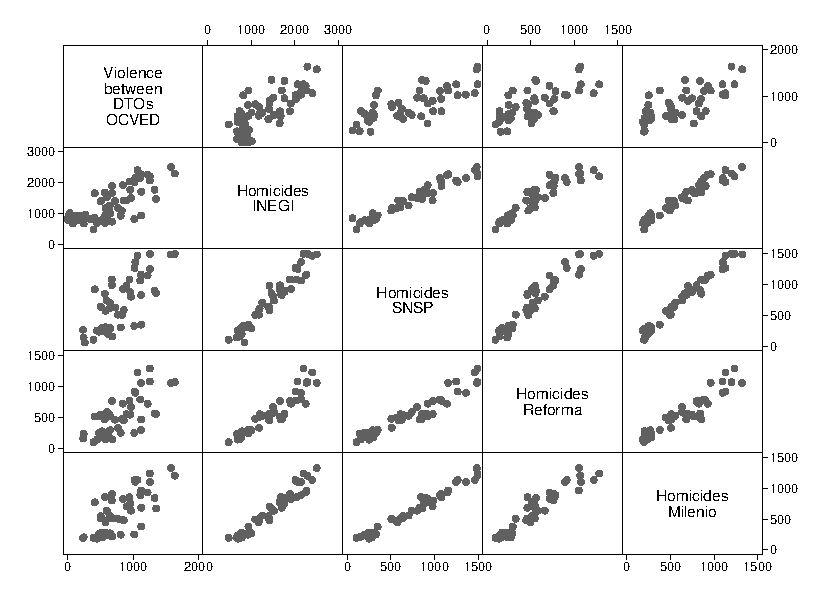
\includegraphics[scale=1]{figures/correlation_homicides.pdf}  
       \caption{Scatter plot of violence among DTOs and homicide data}
       \label{fig:comparison_scatter_homicide}
\end{figure}






%%%%%%%%%%%%%%%%%%%
% Arrests

Table \ref{tab:correlation_non_violence_OCVED_government} reports the correlation between the number of detention events , seizures of dugs, criminal assets and weapons recorded in OCVED and comparable data reported by government authorites. Due to the limited availability of government information on public security, the data used in this table  is aggregated at the national year level. OCVED data on arrests is compared with drug related detentions reported by government authoriteis and the correlation factor (r=0.58) indicates a high degree of congruence between the two metrics. Due to the lack of avaiable official data on drug interdiction, the number of drug seizures recorded in OCVED is contrasted againsts the annual number of metric tons of illicit drugs seized by government authroties. Unfortunately these two units of analysis are not comparable and the correlation factor suggests a weak association (r=0.24). The data on seizures of criminal assets recorded in OCVED includes confiscation of aerial, terrestrial and meritime vehicles as well as real estate. In contrast, government reports only include seizures of these three types of vehicles but there is not data about real estate confiscation from organized criminal groups. Despite these differences, the data on seizures of criminal assets is highly correlated (r=0.92). Finally, the data on seizures of weapons recorded by OCVED and registered by government authorities is also highly correlated (r=0.77). Despite the methodological differences, the correlation analysis provides a high degree of confidence about the validity of the event data comprised in OCVED when compared to official reports. To facilitate the interpretation of these relationsips, the correlation factors are illustrated in Figure \ref{fig:correlation_non_violence_OCVED_government}.



\begin{table}[h!]
\small
%\begin{spacing}{-0.8}
    \caption{Correlation of non-violent event data in OCVED and comparable government data}
    \label{tab:correlation_non_violence_OCVED_government}
%\end{spacing}
\begin{spacing}{0.95}
    \centering
    \begin{tabular}{rccccp{2cm}}
    \hline
 & \multicolumn{4}{c}{Event data in COVED}			\\	

Government data	&	Arrests 	&	Drug seizures 	&	Seizures of assets 	&	Seizures of guns 	\\	\cline{2-5}
Arrests	&	0.5816	&		&		&		\\	
Drug seizures 	&		&	0.2399	&		&		\\	
Vehicles seized 	&		&		&	0.9243	&		\\	
Weapons seized 	&		&		&		&	0.7729	\\	\hline

\end{tabular}
\end{spacing}
\end{table}








%%%%%%%%%%%%%%%%%%%%%%%%%%%%%%%%%%%%%%%%%%%%%%%%%%%%%%%%%%%%%%%%%%%%%%%%%%%%%%%%%%%%%%%%%%%%%%%%%%%%%%%%


\begin{figure}[h]
\centering
\subfigure[Arrests]{
    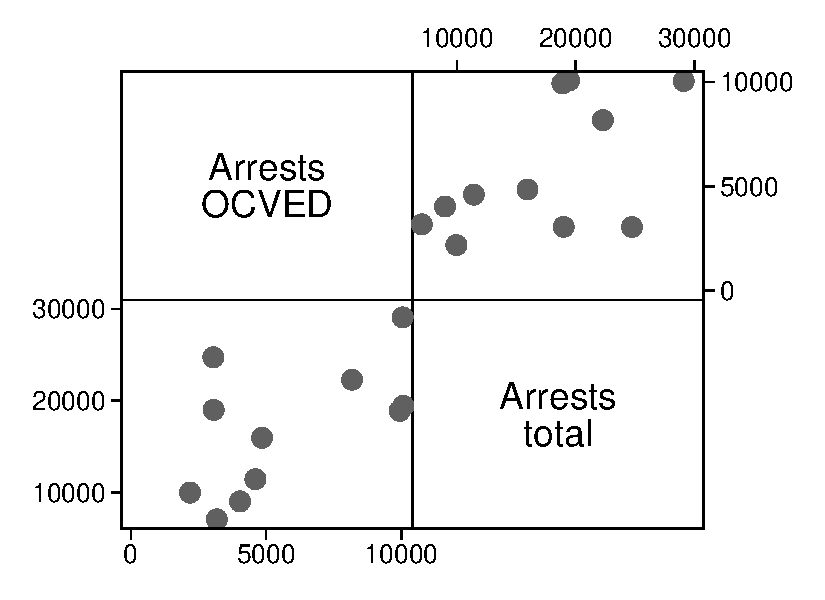
\includegraphics[width=.45\textwidth]{figures/correlation_arrests.pdf}
}
\subfigure[Drug seizures]{
    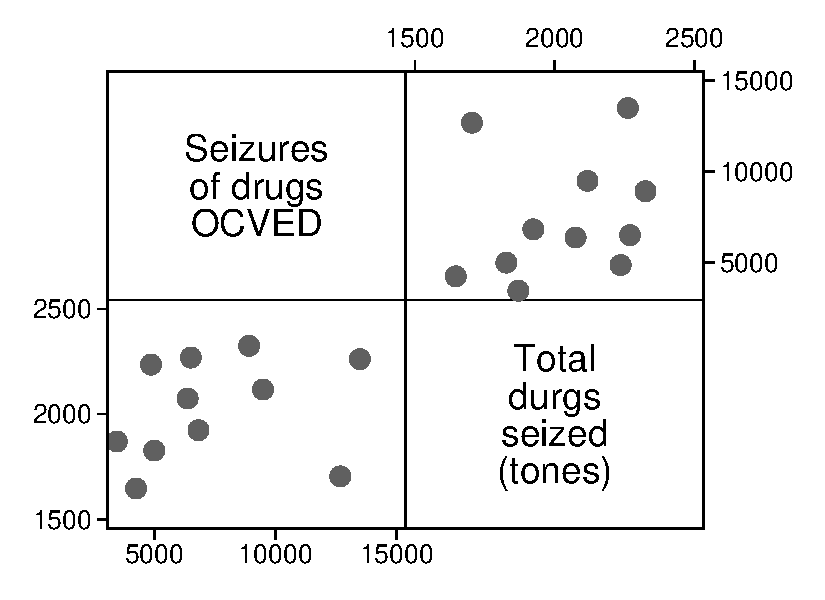
\includegraphics[width=.45\textwidth]{figures/correlation_drugs.pdf}
}
\subfigure[Seizures of assets]{
    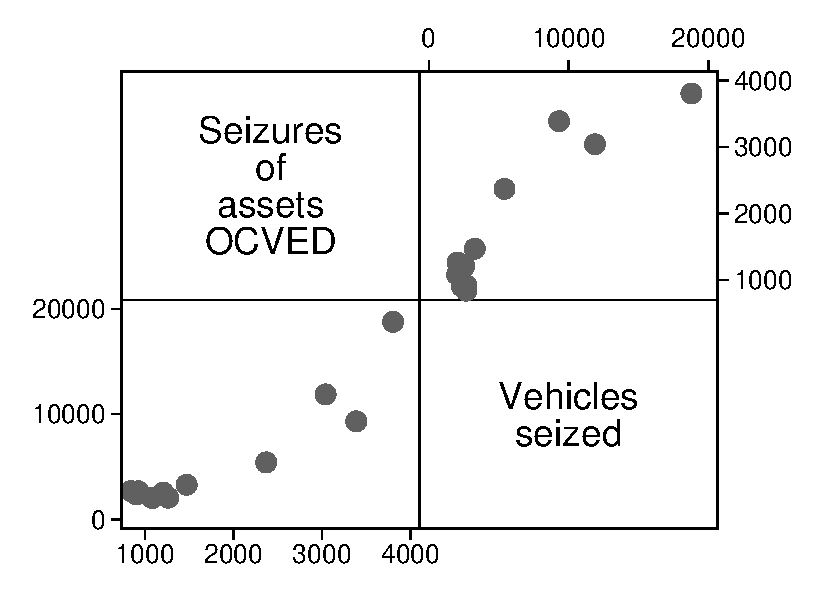
\includegraphics[width=.45\textwidth]{figures/correlation_vehicles.pdf}
}
\subfigure[Seizures of guns]{
    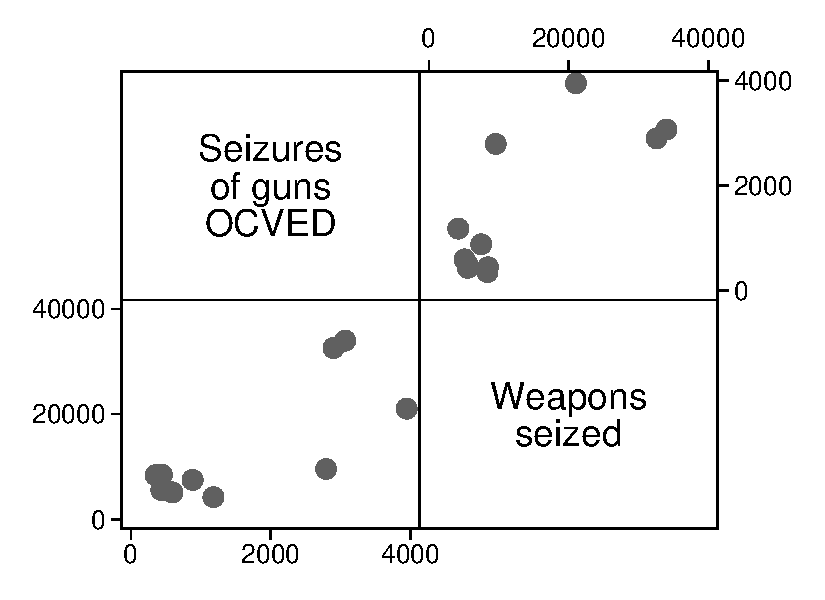
\includegraphics[width=.45\textwidth]{figures/correlation_guns.pdf}
}
\caption{Correlation of non-violent event data in OCVED and comparable government data}
\label{fig:correlation_non_violence_OCVED_government}
\end{figure}





%%%%%%%%%%%%%%%%%%%%%%%%%%%%%%%%%%%%%%%%%%%%%%%%%%%%%%%%%%%%%%%%%%%%%%%%%%%%%%%%%%%%%%%%%%%%%%%%%%%%%%%%
%%%%%%%%%%%%%%%%%%%%%%%%%%%%%%%%%%%%%%%%%%%%%%%%%%%%%%%%%%%%%%%%%%%%%%%%%%%%%%%%%%%%%%%%%%%%%%%%%%%%%%%%
%%%%%%%%%%%%%%%%%%%%%%%%%%%%%%%%%%%%%%%%%%%%%%%%%%%%%%%%%%%%%%%%%%%%%%%%%%%%%%%%%%%%%%%%%%%%%%%%%%%%%%%%
%%%%%%%%%%%%%%%%%%%%%%%%%%%%%%%%%%%%%%%%%%%%%%%%%%%%%%%%%%%%%%%%%%%%%%%%%%%%%%%%%%%%%%%%%%%%%%%%%%%%%%%%




\clearpage

\section{Regression Analysis Robustness Check}


This section replicates the regression analysis presented in the manuscript and reports a variety of additional robustness checks. Table \ref{tab:summary_robustness} summarizes the different model specifications considered in the study. Tables \ref{tab:enforcement_allDTOs_Road_L4L} and \ref{tab:enforcement_MainMinorDTOs_Road_L4L} in the Appendix correspond to Tables 2 and 3 in the article. Tables \ref{tab:enforcement_allDTOs_Road_L2L}-\ref{tab:enforcement_MainMinorDTOs_Road_L8L} offer alternative specifications using different lags for the law enforcement tactics.  Due to the multiple interaction terms, some model specifications could not handle the full list of control variables without generating proglems of overidentification. In those cases, some covariates were excluded. In general, the results provide strong support for the main hypotheses advanced in this research. \\





\begin{table}[h!]
\small
%\begin{spacing}{-0.8}
    \caption{Summary of model specifications for robustness tests}
    \label{tab:summary_robustness}
%\end{spacing}
\begin{spacing}{0.95}
    \centering
    \begin{tabular}{lll}
    \hline
	&	Enforcement data	&	Interaction terms	\\	\hline	\hline
							
\multirow{2}{*}{Table \ref{tab:enforcement_allDTOs_Road_L4L}}	&	\multirow{2}{*}{Lagged 4 weeks}	&	Enforcement tactic $\times$ All DTOs	\\		
	&		&	Enforcement tactic $\times$ Road density 	\\	\hline	
							
\multirow{3}{*}{Table \ref{tab:enforcement_MainMinorDTOs_Road_L4L}}	&	\multirow{3}{*}{Lagged 4 weeks}	&	Enforcement tactic $\times$ Main DTOs	\\		
	&		&	Enforcement tactic $\times$ Secondary DTOs	\\		
	&		&	Enforcement tactic $\times$ Road density 	\\	\hline	
							
\multirow{2}{*}{Table \ref{tab:enforcement_allDTOs_Road_L2L}}	&	\multirow{2}{*}{Lagged 2 weeks}	&	Enforcement tactic $\times$ All DTOs	\\		
	&		&	Enforcement tactic $\times$ Road density 	\\	\hline	
							
\multirow{3}{*}{Table \ref{tab:enforcement_MainMinorDTOs_Road_L2L}}	&	\multirow{3}{*}{Lagged 2 weeks}	&	Enforcement tactic $\times$ Main DTOs	\\		
	&		&	Enforcement tactic $\times$ Secondary DTOs	\\		
	&		&	Enforcement tactic $\times$ Road density 	\\	\hline	
							
\multirow{2}{*}{Table \ref{tab:enforcement_allDTOs_Road_L8L}}	&	\multirow{2}{*}{Lagged 8 weeks}	&	Enforcement tactic $\times$ All DTOs	\\		
	&		&	Enforcement tactic $\times$ Road density 	\\	\hline	
							
\multirow{3}{*}{Table \ref{tab:enforcement_MainMinorDTOs_Road_L8L}}	&	\multirow{3}{*}{Lagged 8 weeks}	&	Enforcement tactic $\times$ Main DTOs	\\		
	&		&	Enforcement tactic $\times$ Secondary DTOs	\\		
	&		&	Enforcement tactic $\times$ Road density 	\\	\hline	

		
\hline
\end{tabular}
\end{spacing}
\end{table}




%%%%%%%%%%%%%%%%%%%%%%%%%%%%%%%%%%%%%%%%%%%%%%%%%%%%%%%%%%%%%%%%%%%%%%%%%%%%%%%%%%%%%%%%%%%%%%%%%%%%%



\begin{landscape}

\begin{center}
\small
\begin{spacing}{0.85}
\begin{longtable}{lccccc}

\caption{Effect of law enforcement (lagged 4 weeks), all DTOs, and road density on violence between DTOs} \label{tab:enforcement_allDTOs_Road_L4L} \\

\hline 
\multicolumn{1}{l}{\textbf{Model }} &\multicolumn{1}{c}{\textbf{1}} & \multicolumn{1}{c}{\textbf{2}} & \multicolumn{1}{c}{\textbf{3}} & \multicolumn{1}{c}{\textbf{4}} & \multicolumn{1}{c}{\textbf{ 5}} \\ \hline 
\endfirsthead


\multicolumn{6}{c}{{\tablename\ \thetable{} -- continued from previous page}} \\ \hline
\multicolumn{1}{l}{\textbf{Model }} &\multicolumn{1}{c}{\textbf{1}} & \multicolumn{1}{c}{\textbf{2}} & \multicolumn{1}{c}{\textbf{3}} & \multicolumn{1}{c}{\textbf{4}} & \multicolumn{1}{c}{\textbf{ 5}} \\ \hline 
\endhead

\hline \multicolumn{6}{c}{{Continued on next page}} \\ \hline
\endfoot

\hline \hline
\endlastfoot

Lambda & 0.172*** & 0.172*** & 0.182*** & 0.175*** & 0.177***  \\ 
 & (0.004)  & (0.004)  & (0.004)  & (0.004)  & (0.004)   \\ 
                 
Violent enforcement (L4L) $\times$ All DTOs & 0.063*** &   &   &   &    \\ 
 & (0.001)  &   &   &   &    \\ 
Arrests  (L4L)  $\times$ All DTOs &   & 0.039*** &   &   &    \\ 
 &   & (0.000)  &   &   &    \\ 
Seizures of drugs  (L4L)  $\times$ All DTOs &   &   & 0.034*** &   &    \\ 
 &   &   & (0.000)  &   &    \\ 
 Seizures of assets  (L4L)  $\times$ All DTOs &   &   &   & 0.055*** &    \\ 
 &   &   &   & (0.000)  &    \\ 
 Seizures of guns  (L4L) $\times$ All DTOs &   &   &   &   & 0.047***  \\ 
 &   &   &   &   & (0.001)   \\ 
                 
Violent enforcement (L4L) $\times$ Road density & -49.222*** &   &   &   &    \\ 
 & (9.015)  &   &   &   &    \\ 
Arrests  (L4L)  $\times$ Road density &   & -12.226*** &   &   &    \\ 
 &   & (2.797)  &   &   &    \\ 
Seizures of drugs  (L4L)  $\times$ Road density &   &   & 20.278*** &   &    \\ 
 &   &   & (2.250)  &   &    \\ 
 Seizures of assets  (L4L)  $\times$ Road density &   &   &   & 2.587  &    \\ 
 &   &   &   & (5.050)  &    \\ 
 Seizures of guns  (L4L) $\times$ Road density &   &   &   &   & -85.494***  \\ 
 &   &   &   &   & (5.427)   \\ 
                 
Violent enforcement  (L4L)  & 0.008$^{\dag}$ &   &   &   &    \\ 
 & (0.004)  &   &   &   &    \\ 
Arrests  (L4L)  &   & -0.014*** &   &   &    \\ 
 &   & (0.001)  &   &   &    \\ 
Seizures of drugs  (L4L)  &   &   & -0.025*** &   &    \\ 
 &   &   & (0.001)  &   &    \\ 
Seizures of assets  (L4L)  &   &   &   & -0.031*** &    \\ 
 &   &   &   & (0.002)  &    \\ 
Seizures of guns  (L4L)  &   &   &   &   & 0.017***  \\ 
 &   &   &   &   & (0.002)   \\ 
                 
                 
                 
All DTOs & 0.077*** & 0.065*** & 0.069*** & 0.073*** & 0.073***  \\ 
 & (0.000)  & (0.000)  & (0.000)  & (0.000)  & (0.000)   \\ 
Road density & -3.844*** & -4.231*** & -4.092*** & -4.395*** & -4.214***  \\ 
 & (0.847)  & (1.031)  & (1.045)  & (0.935)  & (0.966)   \\ 
Drug production area & 0.000  & 0.000  & 0.000  & 0.000  & 0.000  \\ 
 & (0.000)  & (0.000)  & (0.000)  & (0.000)  & (0.000)   \\ 
Gulf & -0.004*** & -0.004** & -0.004** & -0.004*** & -0.004***  \\ 
 & (0.001)  & (0.001)  & (0.001)  & (0.001)  & (0.001)   \\ 
North & 0.017*** & 0.019*** & 0.019*** & 0.018*** & 0.017***  \\ 
 & (0.001)  & (0.002)  & (0.002)  & (0.002)  & (0.002)   \\ 
Pacific & 0.003** & 0.003* & 0.002* & 0.002$^{\dag}$ & 0.002*  \\ 
 & (0.001)  & (0.001)  & (0.001)  & (0.001)  & (0.001)   \\ 
Local drug market & 0.000** & 0.000*** & 0.000*** & 0.000*** & 0.000***  \\ 
 & (0.000)  & (0.000)  & (0.000)  & (0.000)  & (0.000)   \\ 
                 
Rifles & -0.003*** & -0.003*** & -0.003*** & -0.003*** & -0.003***  \\ 
 & (0.001)  & (0.001)  & (0.001)  & (0.001)  & (0.001)   \\ 
Potential cocaine production & 0.000*** & 0.000*** & 0.000*** & 0.000*** & 0.000***  \\ 
 & (0.000)  & (0.000)  & (0.000)  & (0.000)  & (0.000)   \\ 
Corruption & 0.000*** & 0.000*** & 0.000*** & 0.000*** & 0.000***  \\ 
 & (0.000)  & (0.000)  & (0.000)  & (0.000)  & (0.000)   \\ 
Schooling & 0.005*** & 0.006*** & 0.006*** & 0.006*** & 0.006***  \\ 
 & (0.000)  & (0.000)  & (0.000)  & (0.000)  & (0.000)   \\ 
Cocaine price & 0.000*** & 0.000*** & 0.000*** &  &   \\ 
 & (0.000)  & (0.000)  & (0.000)  &  &    \\ 
                 
Poverty & 0.009*** & 0.010*** & 0.010*** & 0.010*** & 0.010***  \\ 
 & (0.000)  & (0.000)  & (0.000)  & (0.000)  & (0.000)   \\ 
Population & 0.002*** & 0.002*** & 0.002*** & 0.002*** & 0.002***  \\ 
 & (0.000)  & (0.000)  & (0.000)  & (0.000)  & (0.000)   \\ 
Rate of violence among DTOs (lagged) & 0.011*** & 0.011*** & 0.011*** & 0.011*** & 0.011***  \\ 
 & (0.000)  & (0.000)  & (0.000)  & (0.000)  & (0.000)   \\ 
Constant & 0.007  & -0.003  & 0.004  & -0.010  & -0.003   \\ 
 & (0.012)  & (0.012)  & (0.012)  & (0.012)  & (0.012)   \\ \hline
                 
Rho & -0.117  & -0.108  & -0.120  & -0.117  & -0.120   \\ 
% Sigma$^{2}V$ & 0.012  & 0.012  & 0.012  & 0.012  & 0.012   \\ 
% Sigma$^{2}V$ & 0.169  & 0.255  & 0.264  & 0.210  & 0.225   \\ 
% Theta & 0.733  & 0.783  & 0.786  & 0.760  & 0.769   \\ 
                 
Observations  &  1,657,800   &  1,657,800   &  1,657,800   &  1,657,800   &  1,657,800    \\ \hline

\multicolumn{6}{l}{``L4L'' refers to event data lagged four weeks and logged.  *** p< 0.001, ** p< 0.01, * p< 0.05, $^{\dag}$ p< 0.1} \\
%\multicolumn{6}{l}{} \\

\end{longtable}
\end{spacing}
\end{center}
%\end{landscape}


%%%%%%%%%%%%%%%%%%%%%%%%%%%%%%%%%%%%%%%%%%%%%%%%%%%%%%%%%%%%%%%%%%%%%%%%%%%%%%%%%%%%%%%%%%%%%%%%%%%%%




%%%%%%%%%%%%%%%%%%%%%%%%%%%%%%%%%%%%%%%%%%%%%%%%%%%%%%%%%%%%%%%%%%%%%%%%%%%%%%%%%%%%%%%%%%%%%%%%%%%%%



%\begin{landscape}
\begin{center}
\small
\begin{spacing}{0.85}
\begin{longtable}{lccccc}

\caption{Effect of law enforcement (lagged 4 weeks), main and secondary DTOs, and road density on violence between DTOs} \label{tab:enforcement_MainMinorDTOs_Road_L4L} \\

\hline 
\multicolumn{1}{l}{\textbf{Model }} &\multicolumn{1}{c}{\textbf{6}} & \multicolumn{1}{c}{\textbf{7}} & \multicolumn{1}{c}{\textbf{8}} & \multicolumn{1}{c}{\textbf{9}} & \multicolumn{1}{c}{\textbf{10}} \\ \hline 
\endfirsthead


\multicolumn{6}{c}{{\tablename\ \thetable{} -- continued from previous page}} \\ \hline
\multicolumn{1}{l}{\textbf{Model }} &\multicolumn{1}{c}{\textbf{6}} & \multicolumn{1}{c}{\textbf{7}} & \multicolumn{1}{c}{\textbf{8}} & \multicolumn{1}{c}{\textbf{9}} & \multicolumn{1}{c}{\textbf{10}} \\ \hline 
\endhead

\hline \multicolumn{6}{c}{{Continued on next page}} \\ \hline
\endfoot

\hline \hline
\endlastfoot

Lambda & 0.167*** & 0.169*** & 0.177*** & 0.171*** & 0.172*** \\ 
 & (0.004) & (0.004) & (0.004) & (0.004) & (0.004) \\ 
Violent enforcement (L4L) $\times$ Main DTOs & 0.096*** & & & & \\ 
 & (0.001) & & & & \\ 
Arrests (L4L) $\times$ Main DTOs & & 0.041*** & & & \\ 
 & & (0.000) & & & \\ 
Seizures of drugs (L4L) $\times$ Main DTOs & & & 0.033*** & & \\ 
 & & & (0.000) & & \\ 
Seizures of assets (L4L) $\times$ Main DTOs & & & & 0.057*** & \\ 
 & & & & (0.001) & \\ 
Seizures of guns (L4L) $\times$ Main DTOs & & & & & 0.054*** \\ 
 & & & & & (0.001) \\ 
 
Violent enforcement (L4L) $\times$ Secondary DTOs & -0.048*** & & & & \\ 
 & (0.002) & & & & \\ 
Arrests (L4L) $\times$ Secondary DTOs & & 0.017*** & & & \\ 
 & & (0.001) & & & \\ 
Seizures of drugs (L4L) $\times$ Secondary DTOs & & & 0.028*** & & \\ 
 & & & (0.001) & & \\ 
Seizures of assets (L4L) $\times$ Secondary DTOs & & & & 0.033*** & \\ 
 & & & & (0.002) & \\ 
Seizures of guns (L4L) $\times$ Secondary DTOs & & & & & 0.007*** \\ 
 & & & & & (0.002) \\ 
 
Violent enforcement (L4L) $\times$ Road density & -45.224*** & & & & \\ 
 & (9.006) & & & & \\ 
Arrests (L4L) $\times$ Road density & & -13.290*** & & & \\ 
 & & (2.799) & & & \\ 
Seizures of drugs (L4L) $\times$ Road density & & & 18.239*** & & \\ 
 & & & (2.251) & & \\ 
Seizures of assets (L4L) $\times$ Road density & & & & 1.425 & \\ 
 & & & & (5.049) & \\ 
Seizures of guns (L4L) $\times$ Road density & & & & & -86.003*** \\ 
 & & & & & (5.430) \\ 
 
Violent enforcement (L4L) & -0.021*** & & & & \\ 
 & (0.004) & & & & \\ 
Arrests (L4L) & & -0.013*** & & & \\ 
 & & (0.001) & & & \\ 
Seizures of drugs (L4L) & & & -0.022*** & & \\ 
 & & & (0.001) & & \\ 
Seizures of assets (L4L) & & & & -0.028*** & \\ 
 & & & & (0.002) & \\ 
Seizures of guns (L4L) & & & & & 0.016*** \\ 
 & & & & & (0.002) \\ 
 
Main DTOs & 0.067*** & 0.058*** & 0.061*** & 0.065*** & 0.064*** \\ 
 & (0.000) & (0.000) & (0.000) & (0.000) & (0.000) \\ 
Secondary DTOs & 0.129*** & 0.109*** & 0.113*** & 0.117*** & 0.123*** \\ 
 & (0.001) & (0.001) & (0.001) & (0.001) & (0.001) \\ 
Road density & -3.374*** & -3.459*** & -3.400** & -3.414*** & -3.223*** \\ 
 & (0.826) & (1.015) & (1.036) & (0.933) & (0.939) \\ 
 
Drug production area & 0.000 & 0.000$^{\dag}$ & 0.000* & 0.000$^{\dag}$ & 0.000 \\ 
 & (0.000) & (0.000) & (0.000) & (0.000) & (0.000) \\ 
Gulf & -0.005*** & -0.004*** & -0.004*** & -0.004*** & -0.005*** \\ 
 & (0.001) & (0.001) & (0.001) & (0.001) & (0.001) \\ 
North & 0.018*** & 0.019*** & 0.019*** & 0.019*** & 0.018*** \\ 
 & (0.001) & (0.002) & (0.002) & (0.002) & (0.002) \\ 
Pacific & 0.003** & 0.003* & 0.003* & 0.002* & 0.003* \\ 
 & (0.001) & (0.001) & (0.001) & (0.001) & (0.001) \\ 
Poverty & 0.008*** & 0.010*** & 0.010*** & 0.009*** & 0.009*** \\ 
 & (0.000) & (0.000) & (0.000) & (0.000) & (0.000) \\ 
Population & 0.002*** & 0.003*** & 0.003*** & 0.002*** & 0.002*** \\ 
 & (0.000) & (0.000) & (0.000) & (0.000) & (0.000) \\ 
Rifles & 0.001 & 0.001 & 0.000 & 0.000 & 0.000 \\ 
 & (0.001) & (0.001) & (0.001) & (0.001) & (0.001) \\ 
Potential cocaine production & 0.000*** & 0.000*** & 0.000*** & 0.000*** & 0.000*** \\ 
 & (0.000) & (0.000) & (0.000) & (0.000) & (0.000) \\ 
Schooling & 0.005*** & 0.006*** & 0.006*** & 0.006*** & 0.006*** \\ 
 & (0.000) & (0.000) & (0.000) & (0.000) & (0.000) \\ 
Rate of violence among DTOs (lagged) & 0.011*** & 0.011*** & 0.011*** & 0.011*** & 0.011*** \\ 
 & (0.000) & (0.000) & (0.000) & (0.000) & (0.000) \\ 
Constant & -0.055*** & -0.061*** & -0.056*** & -0.054*** & -0.048*** \\ 
 & (0.012) & (0.012) & (0.012) & (0.012) & (0.012) \\ \hline
 
Rho & -0.0747 & -0.0722 & -0.0759 & -0.0747 & -0.0769 \\ 
% Sigma$^{2}V$ & 0.0117 & 0.0117 & 0.0117 & 0.0117 & 0.0117 \\ 
% Sigma$^{2}V$ & 0.0001 & 0.0001 & 0.0001 & 0.0001 & 0.0001 \\ 
% Theta & -11.8120 & -11.8660 & -11.8340 & -11.8410 & -11.8870 \\ 
 
Observations & 1,657,800 & 1,657,800 & 1,657,800 & 1,657,800 & 1,657,800 \\ \hline


\hline  
\multicolumn{6}{l}{``L4L'' refers to event data lagged four weeks and logged.  *** p< 0.001, ** p< 0.01, * p< 0.05, $^{\dag}$ p< 0.1} \\
%\multicolumn{6}{l}{} \\
 

\end{longtable}
\end{spacing}
\end{center}
%\end{landscape}



%%%%%%%%%%%%%%%%%%%%%%%%%%%%%%%%%%%%%%%%%%%%%%%%%%%%%%%%%%%%%%%%%%%%%%%%%%%%%%%%%%%%%%%%%%%%%%%%%%%%%



%\begin{landscape}
\begin{center}
\small
\begin{spacing}{0.85}
\begin{longtable}{lccccc}

\caption{Effect of law enforcement (lagged 2 weeks), all DTOs, and road density on violence between DTOs} \label{tab:enforcement_allDTOs_Road_L2L} \\

\hline 
\multicolumn{1}{l}{\textbf{Model }} &\multicolumn{1}{c}{\textbf{11}} & \multicolumn{1}{c}{\textbf{12}} & \multicolumn{1}{c}{\textbf{13}} & \multicolumn{1}{c}{\textbf{14}} & \multicolumn{1}{c}{\textbf{15}} \\ \hline 
\endfirsthead


\multicolumn{6}{c}{{\tablename\ \thetable{} -- continued from previous page}} \\ \hline
\multicolumn{1}{l}{\textbf{Model }} &\multicolumn{1}{c}{\textbf{11}} & \multicolumn{1}{c}{\textbf{12}} & \multicolumn{1}{c}{\textbf{13}} & \multicolumn{1}{c}{\textbf{14}} & \multicolumn{1}{c}{\textbf{15}} \\ \hline 
\endhead

\hline \multicolumn{6}{c}{{Continued on next page}} \\ \hline
\endfoot

\hline \hline
\endlastfoot
                
Lambda  & 0.177*** & 0.170*** & 0.181*** & 0.174*** & 0.173*** \\
 & (0.004)  & (0.004)  & (0.004)  & (0.004)  & (0.004)  \\
                
Violent enforcement (L2L) $\times$ All DTOs & 0.054*** &   &   &   &   \\
 & (0.001)  &   &   &   &   \\
Arrests (L2L) $\times$ All DTOs &   & 0.041*** &   &   &   \\
 &   & (0.000)  &   &   &   \\
Seizures of drugs (L2L) $\times$ All DTOs &   &   & 0.033*** &   &   \\
 &   &   & (0.000)  &   &   \\
Seizures of assets (L2L) $\times$ All DTOs &   &   &   & 0.055*** &   \\
 &   &   &   & (0.000)  &   \\
Seizures of guns (L2L) $\times$ All DTOs &   &   &   &   & 0.049*** \\
 &   &   &   &   & (0.001)  \\
                
Violent enforcement (L2L) $\times$ Road density & -128.830*** &   &   &   &   \\
 & (8.862)  &   &   &   &   \\
Arrests (L2L) $\times$ Road density &   & -7.409** &   &   &   \\
 &   & (2.784)  &   &   &   \\
Seizures of drugs (L2L) $\times$ Road density &   &   & 17.080*** &   &   \\
 &   &   & (2.247)  &   &   \\
Seizures of assets (L2L) $\times$ Road density &   &   &   & -14.453** &   \\
 &   &   &   & (5.002)  &   \\
Seizures of guns (L2L) $\times$ Road density &   &   &   &   & -50.821*** \\
 &   &   &   &   & (5.418)  \\
                
Violent enforcement (L2L)  & 0.077*** &   &   &   &   \\
 & (0.004)  &   &   &   &   \\
Arrests (L2L)  &   & -0.018*** &   &   &   \\
 &   & (0.001)  &   &   &   \\
Seizures of drugs (L2L)  &   &   & -0.026*** &   &   \\
 &   &   & (0.001)  &   &   \\
Seizures of assets (L2L) &   &   &   & -0.027*** &   \\
 &   &   &   & (0.002)  &   \\
Seizures of guns (L2L)  &   &   &   &   & 0.003  \\
 &   &   &   &   & (0.002)  \\
                
                
All DTOS & 0.077*** & 0.064*** & 0.069*** & 0.073*** & 0.073*** \\
 & (0.000)  & (0.000)  & (0.000)  & (0.000)  & (0.000)  \\
                
Road density & -4.129*** & -4.804*** & -4.489*** & -4.380*** & -4.307*** \\
 & (0.837)  & (1.040)  & (1.050)  & (0.928)  & (0.979)  \\

Drug production area & 0.000  & 0.000  & 0.000  & 0.000  & 0.000  \\
 & (0.000)  & (0.000)  & (0.000)  & (0.000)  & (0.000)  \\
Gulf & -0.004*** & -0.004** & -0.004** & -0.004*** & -0.004*** \\
 & (0.001)  & (0.001)  & (0.001)  & (0.001)  & (0.001)  \\
North & 0.016*** & 0.019*** & 0.019*** & 0.018*** & 0.018*** \\
 & (0.001)  & (0.002)  & (0.002)  & (0.002)  & (0.002)  \\
Pacific & 0.002* & 0.002* & 0.002$^{\dag}$& 0.002$^{\dag}$& 0.002* \\
 & (0.001)  & (0.001)  & (0.001)  & (0.001)  & (0.001)  \\
Poverty & 0.009*** & 0.011*** & 0.011*** & 0.010*** & 0.010*** \\
 & (0.000)  & (0.000)  & (0.000)  & (0.000)  & (0.000)  \\
Population & 0.002*** & 0.002*** & 0.002*** & 0.002*** & 0.002*** \\
 & (0.000)  & (0.000)  & (0.000)  & (0.000)  & (0.000)  \\
Corruption & 0.000*** & 0.000*** & 0.000*** & 0.000*** & 0.000*** \\
 & (0.000)  & (0.000)  & (0.000)  & (0.000)  & (0.000)  \\
Local drug markets & 0.000** & 0.000*** & 0.000*** & 0.000*** & 0.000*** \\
 & (0.000)  & (0.000)  & (0.000)  & (0.000)  & (0.000)  \\
Rifles & -0.003** & -0.002* & -0.003*** & -0.002** & -0.003*** \\
 & (0.001)  & (0.001)  & (0.001)  & (0.001)  & (0.001)  \\
                
Potential cocaine production & 0.000*** & 0.000*** & 0.000*** & 0.000*** & 0.000*** \\
 & (0.000)  & (0.000)  & (0.000)  & (0.000)  & (0.000)  \\
Schooling & 0.006*** & 0.007*** & 0.006*** & 0.006*** & 0.006*** \\
 & (0.000)  & (0.000)  & (0.000)  & (0.000)  & (0.000)  \\
Rate of violence among DTOs (lagged) & 0.014*** & 0.014*** & 0.013*** & 0.013*** & 0.013*** \\
 & (0.000)  & (0.000)  & (0.000)  & (0.000)  & (0.000)  \\
                
Constant & -0.008  & -0.023$^{\dag}$& -0.011  & -0.011  & -0.006  \\
 & (0.011)  & (0.012)  & (0.012)  & (0.012)  & (0.012)  \\ \hline
                
Rho & -0.124  & -0.104  & -0.117  & -0.115  & -0.113  \\
% Sigma^2_v & 0.012  & 0.012  & 0.012  & 0.012  & 0.012  \\
% Sigma^2_1 & 0.167  & 0.262  & 0.268  & 0.207  & 0.232  \\
%Theta & 0.732  & 0.786  & 0.788  & 0.759  & 0.772  \\
                
Observations  & 1,662,712  & 1,662,712  & 1,662,712  & 1,662,712  & 1,662,712  \\

\hline  
\multicolumn{6}{l}{``L2L'' refers to event data lagged two weeks and logged.  *** p< 0.001, ** p< 0.01, * p< 0.05, $^{\dag}$ p< 0.1} \\
%\multicolumn{6}{l}{} \\
 
\end{longtable}
\end{spacing}
\end{center}
%\end{landscape}



%%%%%%%%%%%%%%%%%%%%%%%%%%%%%%%%%%%%%%%%%%%%%%%%%%%%%%%%%%%%%%%%%%%%%%%%%%%%%%%%%%%%%%%%%%%%%%%%%%%%%



%\begin{landscape}
\begin{center}
\small
\begin{spacing}{0.85}
\begin{longtable}{lccccc}

\caption{Effect of law enforcement (lagged 2 weeks), main and secondary DTOs, and road density on violence between DTOs} \label{tab:enforcement_MainMinorDTOs_Road_L2L} \\

\hline 
\multicolumn{1}{l}{\textbf{Model }} &\multicolumn{1}{c}{\textbf{16}} & \multicolumn{1}{c}{\textbf{17}} & \multicolumn{1}{c}{\textbf{18}} & \multicolumn{1}{c}{\textbf{19}} & \multicolumn{1}{c}{\textbf{20}} \\ \hline 
\endfirsthead


\multicolumn{6}{c}{{\tablename\ \thetable{} -- continued from previous page}} \\ \hline
\multicolumn{1}{l}{\textbf{Model }} &\multicolumn{1}{c}{\textbf{16}} & \multicolumn{1}{c}{\textbf{17}} & \multicolumn{1}{c}{\textbf{18}} & \multicolumn{1}{c}{\textbf{19}} & \multicolumn{1}{c}{\textbf{20}} \\ \hline 
\endhead

\hline \multicolumn{6}{c}{{Continued on next page}} \\ \hline
\endfoot

\hline \hline
\endlastfoot
                
Lambda  & 0.170*** & 0.166*** & 0.176*** & 0.169*** & 0.167*** \\
 & (0.004)  & (0.004)  & (0.004)  & (0.004)  & (0.004)  \\
      
Violent enforcement (L2L) $\times$ Main DTOs & 0.085*** &   &   &   &   \\
 & (0.001)  &   &   &   &   \\
Arrests (L2L) $\times$ Main DTOs &   & 0.046*** &   &   &   \\
 &   & (0.000)  &   &   &   \\
Seizures of drugs (L2L) $\times$ Main DTOs &   &   & 0.032*** &   &   \\
 &   &   & (0.000)  &   &   \\
Seizures of assets (L2L) $\times$ Main DTOs &   &   &   & 0.058*** &   \\
 &   &   &   & (0.001)  &   \\
Seizures of guns (L2L) $\times$ Main DTOs &   &   &   &   & 0.057*** \\
 &   &   &   &   & (0.001)  \\

Violent enforcement (L2L) $\times$ Secondary DTOs & -0.050*** &   &   &   &   \\
 & (0.002)  &   &   &   &   \\
Arrests (L2L) $\times$ Secondary DTOs &   & 0.008*** &   &   &   \\
 &   & (0.001)  &   &   &   \\
Seizures of drugs (L2L) $\times$ Secondary DTOs &   &   & 0.026*** &   &   \\
 &   &   & (0.001)  &   &   \\
Seizures of assets (L2L) $\times$ Secondary DTOs &   &   &   & 0.028*** &   \\
 &   &   &   & (0.002)  &   \\
Seizures of guns (L2L) $\times$ Secondary DTOs &   &   &   &   & 0.007*** \\
 &   &   &   &   & (0.002)  \\
                
Violent enforcement (L2L) $\times$ Road density & -125.880*** &   &   &   &   \\
 & (8.854)  &   &   &   &   \\
Arrests (L2L) $\times$ Road density &   & -7.122* &   &   &   \\
 &   & (2.785)  &   &   &   \\
Seizures of drugs (L2L) $\times$ Road density &   &   & 15.199*** &   &   \\
 &   &   & (2.248)  &   &   \\
Seizures of assets (L2L) $\times$ Road density &   &   &   & -15.306** &   \\
 &   &   &   & (5.001)  &   \\
Seizures of guns (L2L) $\times$ Road density &   &   &   &   & -50.804*** \\
 &   &   &   &   & (5.420)  \\
                
Violent enforcement (L2L)  & 0.051*** &   &   &   &   \\
 & (0.004)  &   &   &   &   \\
Arrests (L2L)  &   & -0.019*** &   &   &   \\
 &   & (0.001)  &   &   &   \\
Seizures of drugs (L2L)  &   &   & -0.023*** &   &   \\
 &   &   & (0.001)  &   &   \\
Seizures of assets (L2L) &   &   &   & -0.026*** &   \\
 &   &   &   & (0.002)  &   \\
Seizures of guns (L2L)  &   &   &   &   & 0.001  \\
 &   &   &   &   & (0.002)  \\
                
Main DTOs & 0.067*** & 0.056*** & 0.061*** & 0.065*** & 0.064*** \\
 & (0.000)  & (0.000)  & (0.000)  & (0.000)  & (0.000)  \\
Secondary DTOs & 0.129*** & 0.112*** & 0.114*** & 0.118*** & 0.123*** \\
 & (0.001)  & (0.001)  & (0.001)  & (0.001)  & (0.001)  \\
Road density & -3.261*** & -3.522*** & -3.367** & -3.397*** & -3.287*** \\
 & (0.821)  & (1.030)  & (1.045)  & (0.926)  & (0.952)  \\
Drug production area & 0.000  & 0.000$^{\dag}$& 0.000* & 0.000$^{\dag}$& 0.000  \\
 & (0.000)  & (0.000)  & (0.000)  & (0.000)  & (0.000)  \\
Gulf & -0.004*** & -0.004*** & -0.004*** & -0.004*** & -0.004*** \\
 & (0.001)  & (0.001)  & (0.001)  & (0.001)  & (0.001)  \\
North & 0.017*** & 0.019*** & 0.019*** & 0.019*** & 0.018*** \\
 & (0.001)  & (0.002)  & (0.002)  & (0.002)  & (0.002)  \\
Pacific & 0.003** & 0.003* & 0.003* & 0.002* & 0.003* \\
 & (0.001)  & (0.001)  & (0.001)  & (0.001)  & (0.001)  \\
Poverty & 0.008*** & 0.010*** & 0.010*** & 0.009*** & 0.009*** \\
 & (0.000)  & (0.000)  & (0.000)  & (0.000)  & (0.000)  \\
Population & 0.002*** & 0.003*** & 0.003*** & 0.002*** & 0.002*** \\
 & (0.000)  & (0.000)  & (0.000)  & (0.000)  & (0.000)  \\
                
Rifles & 0.001  & 0.001  & 0.000  & 0.000  & 0.000  \\
 & (0.001)  & (0.001)  & (0.001)  & (0.001)  & (0.001)  \\
               
Potential cocaine production & 0.000*** & 0.000*** & 0.000*** & 0.000*** & 0.000*** \\
 & (0.000)  & (0.000)  & (0.000)  & (0.000)  & (0.000)  \\
Schooling & 0.005*** & 0.006*** & 0.006*** & 0.006*** & 0.006*** \\
 & (0.000)  & (0.000)  & (0.000)  & (0.000)  & (0.000)  \\
Rate of violence among DTOs (lagged) & 0.014*** & 0.014*** & 0.013*** & 0.013*** & 0.013*** \\
 & (0.000)  & (0.000)  & (0.000)  & (0.000)  & (0.000)  \\
             
Constant & -0.054*** & -0.064*** & -0.057*** & -0.055*** & -0.052*** \\
 & (0.011)  & (0.012)  & (0.012)  & (0.012)  & (0.012)  \\ \hline
            
Rho & -0.117  & -0.100  & -0.110  & -0.109  & -0.107  \\
% Sigma^2_v & 0.012  & 0.012  & 0.012  & 0.012  & 0.012  \\
% Sigma^2_1 & 0.162  & 0.259  & 0.268  & 0.208  & 0.220  \\
%Theta & 0.728  & 0.785  & 0.788  & 0.760  & 0.767  \\
                
Observations  & 1,662,712  & 1,662,712  & 1,662,712  & 1,662,712  & 1,662,712  \\

\hline  
\multicolumn{6}{l}{``L2L'' refers to event data lagged two weeks and logged.  *** p< 0.001, ** p< 0.01, * p< 0.05, $^{\dag}$ p< 0.1} \\
%\multicolumn{6}{l}{} \\
 
\end{longtable}
\end{spacing}
\end{center}
%\end{landscape}



%%%%%%%%%%%%%%%%%%%%%%%%%%%%%%%%%%%%%%%%%%%%%%%%%%%%%%%%%%%%%%%%%%%%%%%%%%%%%%%%%%%%%%%%%%%%%%%%%%%%%



%\begin{landscape}
\begin{center}
\small
\begin{spacing}{0.85}
\begin{longtable}{lccccc}

\caption{Effect of law enforcement (lagged 8 weeks), all DTOs, and road density on violence between DTOs} \label{tab:enforcement_allDTOs_Road_L8L} \\

\hline 
\multicolumn{1}{l}{\textbf{Model }} &\multicolumn{1}{c}{\textbf{21}} & \multicolumn{1}{c}{\textbf{22}} & \multicolumn{1}{c}{\textbf{23}} & \multicolumn{1}{c}{\textbf{24}} & \multicolumn{1}{c}{\textbf{25}} \\ \hline 
\endfirsthead


\multicolumn{6}{c}{{\tablename\ \thetable{} -- continued from previous page}} \\ \hline
\multicolumn{1}{l}{\textbf{Model }} &\multicolumn{1}{c}{\textbf{21}} & \multicolumn{1}{c}{\textbf{22}} & \multicolumn{1}{c}{\textbf{23}} & \multicolumn{1}{c}{\textbf{24}} & \multicolumn{1}{c}{\textbf{25}} \\ \hline 
\endhead

\hline \multicolumn{6}{c}{{Continued on next page}} \\ \hline
\endfoot

\hline \hline
\endlastfoot
                
Lambda  & 0.174*** & 0.174*** & 0.187*** & 0.178*** & 0.170*** \\
 & (0.004)  & (0.004)  & (0.004)  & (0.004)  & (0.004)  \\
                
Violent enforcement (L8L) $\times$ All DTOs & 0.053*** &   &   &   &   \\
 & (0.001)  &   &   &   &   \\
Arrests (L8L) $\times$ All DTOs &   & 0.038*** &   &   &   \\
 &   & (0.000)  &   &   &   \\
Seizures of drugs (L8L) $\times$ All DTOs &   &   & 0.032*** &   &   \\
 &   &   & (0.000)  &   &   \\
Seizures of assets (L8L) $\times$ All DTOs &   &   &   & 0.054*** &   \\
 &   &   &   & (0.000)  &   \\
Seizures of guns (L8L) $\times$ All DTOs &   &   &   &   & 0.048*** \\
 &   &   &   &   & (0.001)  \\

Violent enforcement (L8L) $\times$ Road density & -138.870*** &   &   &   &   \\
 & (9.079)  &   &   &   &   \\
Arrests (L8L) $\times$ Road density &   & -5.866* &   &   &   \\
 &   & (2.820)  &   &   &   \\
Seizures of drugs (L8L) $\times$ Road density &   &   & 21.265*** &   &   \\
 &   &   & (2.261)  &   &   \\
Seizures of assets (L8L) $\times$ Road density &   &   &   & 10.864* &   \\
 &   &   &   & (5.087)  &   \\
Seizures of guns (L8L) $\times$ Road density &   &   &   &   & -45.202*** \\
 &   &   &   &   & (5.468)  \\
                
Violent enforcement (L8L)  & 0.054*** &   &   &   &   \\
 & (0.004)  &   &   &   &   \\
Arrests (L8L)  &   & -0.028*** &   &   &   \\
 &   & (0.001)  &   &   &   \\
Seizures of drugs (L8L)  &   &   & -0.033*** &   &   \\
 &   &   & (0.001)  &   &   \\
Seizures of assets (L8L) &   &   &   & -0.042*** &   \\
 &   &   &   & (0.002)  &   \\
Seizures of guns (L8L)  &   &   &   &   & -0.002  \\
 &   &   &   &   & (0.002)  \\
                
All DTOS & 0.077*** & 0.066*** & 0.069*** & 0.073*** & 0.073*** \\
 & (0.000)  & (0.000)  & (0.000)  & (0.000)  & (0.000)  \\
               
Road density & -3.739*** & -4.270*** & -4.110*** & -4.371*** & -4.364*** \\
 & (0.842)  & (1.056)  & (1.063)  & (0.949)  & (0.986)  \\

Drug production area & 0.000  & 0.000  & 0.000  & 0.000  & 0.000  \\
 & (0.000)  & (0.000)  & (0.000)  & (0.000)  & (0.000)  \\
Gulf & -0.004*** & -0.004** & -0.004** & -0.004*** & -0.004*** \\
 & (0.001)  & (0.001)  & (0.001)  & (0.001)  & (0.001)  \\
North & 0.017*** & 0.020*** & 0.020*** & 0.018*** & 0.018*** \\
 & (0.001)  & (0.002)  & (0.002)  & (0.002)  & (0.002)  \\
Pacific & 0.003** & 0.003* & 0.003* & 0.002$^{\dag}$& 0.002* \\
 & (0.001)  & (0.001)  & (0.001)  & (0.001)  & (0.001)  \\
Poverty & 0.008*** & 0.010*** & 0.010*** & 0.010*** & 0.010*** \\
 & (0.000)  & (0.000)  & (0.000)  & (0.000)  & (0.000)  \\
Population & 0.002*** & 0.002*** & 0.002*** & 0.002*** & 0.002*** \\
 & (0.000)  & (0.000)  & (0.000)  & (0.000)  & (0.000)  \\
Corruption & 0.000*** & 0.000*** & 0.000*** & 0.000*** & 0.000*** \\
 & (0.000)  & (0.000)  & (0.000)  & (0.000)  & (0.000)  \\
Local drug markets & 0.000** & 0.000*** & 0.000*** & 0.000*** & 0.000*** \\
 & (0.000)  & (0.000)  & (0.000)  & (0.000)  & (0.000)  \\
Rifles & -0.003*** & -0.003*** & -0.003*** & -0.003** & -0.003*** \\
 & (0.001)  & (0.001)  & (0.001)  & (0.001)  & (0.001)  \\
Cocaine price & 0.000*** & 0.000*** & 0.000*** &   &   \\
 & (0.000)  & (0.000)  & (0.000)  &   &   \\
Potential cocaine production & 0.000*** & 0.000*** & 0.000*** & 0.000*** & 0.000*** \\
 & (0.000)  & (0.000)  & (0.000)  & (0.000)  & (0.000)  \\
Schooling & 0.005*** & 0.006*** & 0.006*** & 0.006*** & 0.006*** \\
 & (0.000)  & (0.000)  & (0.000)  & (0.000)  & (0.000)  \\
Rate of violence among DTOs (lagged) & 0.012*** & 0.012*** & 0.012*** & 0.012*** & 0.012*** \\
 & (0.000)  & (0.000)  & (0.000)  & (0.000)  & (0.000)  \\
                
Constant & 0.009  & -0.007  & 0.001  & -0.011  & -0.007  \\
 & (0.012)  & (0.012)  & (0.012)  & (0.012)  & (0.012)  \\ \hline
                
Rho & -0.121  & -0.109  & -0.124  & -0.120  & -0.110  \\
% Sigma^2_v & 0.012  & 0.012  & 0.012  & 0.012  & 0.012  \\
% Sigma^2_1 & 0.166  & 0.266  & 0.272  & 0.215  & 0.232  \\
%Theta & 0.730  & 0.787  & 0.789  & 0.763  & 0.772  \\
                
Observations  & 1,647,976  & 1,647,976  & 1,647,976  & 1,647,976  & 1,647,976  \\

\hline  
\multicolumn{6}{l}{``L8L'' refers to event data lagged eight weeks and logged.  *** p< 0.001, ** p< 0.01, * p< 0.05, $^{\dag}$ p< 0.1} \\
%\multicolumn{6}{l}{} \\
 
\end{longtable}
\end{spacing}
\end{center}
%\end{landscape}







%%%%%%%%%%%%%%%%%%%%%%%%%%%%%%%%%%%%%%%%%%%%%%%%%%%%%%%%%%%%%%%%%%%%%%%%%%%%%%%%%%%%%%%%%%%%%%%%%%%%%



%\begin{landscape}
\begin{center}
\small
\begin{spacing}{0.85}
\begin{longtable}{lccccc}

\caption{Effect of law enforcement (lagged 8 weeks), main and secondary DTOs, and road density on violence between DTOs} \label{tab:enforcement_MainMinorDTOs_Road_L8L} \\

\hline 
\multicolumn{1}{l}{\textbf{Model }} &\multicolumn{1}{c}{\textbf{26}} & \multicolumn{1}{c}{\textbf{27}} & \multicolumn{1}{c}{\textbf{28}} & \multicolumn{1}{c}{\textbf{29}} & \multicolumn{1}{c}{\textbf{30}} \\ \hline 
\endfirsthead


\multicolumn{6}{c}{{\tablename\ \thetable{} -- continued from previous page}} \\ \hline
\multicolumn{1}{l}{\textbf{Model }} &\multicolumn{1}{c}{\textbf{26}} & \multicolumn{1}{c}{\textbf{27}} & \multicolumn{1}{c}{\textbf{28}} & \multicolumn{1}{c}{\textbf{29}} & \multicolumn{1}{c}{\textbf{30}} \\ \hline 
\endhead

\hline \multicolumn{6}{c}{{Continued on next page}} \\ \hline
\endfoot

\hline \hline
\endlastfoot

                
Lambda  & 0.167*** & 0.171*** & 0.181*** & 0.174*** & 0.166*** \\
 & (0.004)  & (0.004)  & (0.004)  & (0.004)  & (0.004)  \\

Violent enforcement (L8L) $\times$ Main DTOs & 0.061*** &   &   &   &   \\
 & (0.001)  &   &   &   &   \\
Arrests (L8L) $\times$ Main DTOs &   & 0.038*** &   &   &   \\
 &   & (0.000)  &   &   &   \\
Seizures of drugs (L8L) $\times$ Main DTOs &   &   & 0.032*** &   &   \\
 &   &   & (0.000)  &   &   \\
Seizures of assets (L8L) $\times$ Main DTOs &   &   &   & 0.055*** &   \\
 &   &   &   & (0.001)  &   \\
Seizures of guns (L8L) $\times$ Main DTOs &   &   &   &   & 0.054*** \\
 &   &   &   &   & (0.001)  \\
 
Violent enforcement (L8L) $\times$ Secondary DTOs & 0.008*** &   &   &   &   \\
 & (0.002)  &   &   &   &   \\
Arrests (L8L) $\times$ Secondary DTOs &   & 0.024*** &   &   &   \\
 &   & (0.001)  &   &   &   \\
Seizures of drugs (L8L) $\times$ Secondary DTOs &   &   & 0.021*** &   &   \\
 &   &   & (0.001)  &   &   \\
Seizures of assets (L8L) $\times$ Secondary DTOs &   &   &   & 0.033*** &   \\
 &   &   &   & (0.002)  &   \\
Seizures of guns (L8L) $\times$ Secondary DTOs &   &   &   &   & 0.013*** \\
 &   &   &   &   & (0.002)  \\
                
Violent enforcement (L8L) $\times$ Road density & -141.030*** &   &   &   &   \\
 & (9.074)  &   &   &   &   \\
Arrests (L8L) $\times$ Road density &   & -7.831** &   &   &   \\
 &   & (2.821)  &   &   &   \\
Seizures of drugs (L8L) $\times$ Road density &   &   & 19.740*** &   &   \\
 &   &   & (2.263)  &   &   \\
Seizures of assets (L8L) $\times$ Road density &   &   &   & 9.599 . &   \\
 &   &   &   & (5.086)  &   \\
Seizures of guns (L8L) $\times$ Road density &   &   &   &   & -46.311*** \\
 &   &   &   &   & (5.470)  \\
                
Violent enforcement (L8L)  & 0.053*** &   &   &   &   \\
 & (0.004)  &   &   &   &   \\
Arrests (L8L)  &   & -0.025*** &   &   &   \\
 &   & (0.001)  &   &   &   \\
Seizures of drugs (L8L)  &   &   & -0.030*** &   &   \\
 &   &   & (0.001)  &   &   \\
Seizures of assets (L8L) &   &   &   & -0.039*** &   \\
 &   &   &   & (0.002)  &   \\
Seizures of guns (L8L)  &   &   &   &   & -0.001  \\
 &   &   &   &   & (0.002)  \\

Main DTOs & 0.069*** & 0.059*** & 0.061*** & 0.065*** & 0.064*** \\
 & (0.000)  & (0.000)  & (0.000)  & (0.000)  & (0.000)  \\
Secondary DTOs & 0.125*** & 0.107*** & 0.116*** & 0.118*** & 0.121*** \\
 & (0.001)  & (0.001)  & (0.001)  & (0.001)  & (0.001)  \\
Road density & -3.312*** & -3.495*** & -3.481*** & -3.395*** & -3.339*** \\
 & (0.820)  & (1.040)  & (1.053)  & (0.946)  & (0.962)  \\
Drug production area & 0.000  & 0.000$^{\dag}$ & 0.000* & 0.000$^{\dag}$ & 0.000  \\
 & (0.000)  & (0.000)  & (0.000)  & (0.000)  & (0.000)  \\
Gulf & -0.005*** & -0.005*** & -0.004*** & -0.005*** & -0.005*** \\
 & (0.001)  & (0.001)  & (0.001)  & (0.001)  & (0.001)  \\
North & 0.017*** & 0.020*** & 0.020*** & 0.019*** & 0.018*** \\
 & (0.001)  & (0.002)  & (0.002)  & (0.002)  & (0.002)  \\
Pacific & 0.003** & 0.003* & 0.003* & 0.002* & 0.003* \\
 & (0.001)  & (0.001)  & (0.001)  & (0.001)  & (0.001)  \\
Poverty & 0.008*** & 0.010*** & 0.010*** & 0.009*** & 0.009*** \\
 & (0.000)  & (0.000)  & (0.000)  & (0.000)  & (0.000)  \\
Population & 0.002*** & 0.003*** & 0.003*** & 0.002*** & 0.002*** \\
 & (0.000)  & (0.000)  & (0.000)  & (0.000)  & (0.000)  \\

Rifles &   & 0.001  &   & 0.000  & 0.000  \\
 &   & (0.001)  &   & (0.001)  & (0.001)  \\

Potential cocaine production & 0.000*** & 0.000*** & 0.000*** & 0.000*** & 0.000*** \\
 & (0.000)  & (0.000)  & (0.000)  & (0.000)  & (0.000)  \\
Schooling & 0.005*** & 0.006*** & 0.006*** & 0.006*** & 0.006*** \\
 & (0.000)  & (0.000)  & (0.000)  & (0.000)  & (0.000)  \\
Rate of violence among DTOs (lagged) & 0.012*** & 0.012*** & 0.012*** & 0.012*** & 0.012*** \\
 & (0.000)  & (0.000)  & (0.000)  & (0.000)  & (0.000)  \\

Constant & -0.045*** & -0.066*** & -0.051*** & -0.055*** & -0.052*** \\
 & (0.002)  & (0.012)  & (0.003)  & (0.012)  & (0.012)  \\ \hline

Rho & -0.113  & -0.105  & -0.118  & -0.114  & -0.104  \\
% Sigma^2_v & 0.012  & 0.012  & 0.012  & 0.012  & 0.012  \\
% Sigma^2_1 & 0.160  & 0.262  & 0.271  & 0.216  & 0.223  \\
%Theta & 0.725  & 0.785  & 0.789  & 0.763  & 0.767  \\
                
Observations  & 1,647,976  & 1,647,976  & 1,647,976  & 1,647,976  & 1,647,976  \\

\hline  
\multicolumn{6}{l}{``L8L'' refers to event data lagged eight weeks and logged.  *** p< 0.001, ** p< 0.01, * p< 0.05, $^{\dag}$ p< 0.1} \\
%\multicolumn{6}{l}{} \\
 
\end{longtable}
\end{spacing}
\end{center}
\end{landscape}




%%%%%%%%%%%%%%%%%%%%%%%%%%%%%%%%%%%%%%%%%%%%%%
%%%%%%%%%%%%%%%%%%%%%%%%%%%%%%%%%%%%%%%%%%%%%%
%%
%% REFERENCES HERE
%%
%%%%%%%%%%%%%%%%%%%%%%%%%%%%%%%%%%%%%%%%%%%%%%
%%%%%%%%%%%%%%%%%%%%%%%%%%%%%%%%%%%%%%%%%%%%%%

\clearpage

%\begin{singlespace}
\newpage \bibliographystyle{apsr}
\bibliography{Spatial.bib}
%\end{singlespace}



\end{document}

